\chapter{semisimple Lie algebras}
\section{semisimple and reductive Lie algebras}
\begin{itemize}
	\item \textbf{def.:} a complex Lie algebra is \textbf{reductive} if there exists a \textbf{compact} Lie group $K$ s.t.,
	\begin{equation} \label{6.1.1}
		\mathfrak{g} \simeq \mathfrak{k}_\mathbb{C}
	\end{equation}
	\begin{itemize}
		\item an alternate def. from Wikipedia: a Lie algebra is reductive if its adjoint rep. is completely reducible.
	\end{itemize}
	
	\begin{tcolorbox}[title=proof of equivalence:]
		$\Longrightarrow$, complexification of a compact Lie group is reductive:
		\begin{itemize}
			\item the adjoint rep. of a compact Lie group is completely reducible, so is its complexification (they have the same invariant subspaces, $W, W^\perp$, only complexificated).
		\end{itemize}
		
		\noindent\rule[0.5ex]{\linewidth}{0.5pt} % horizontal line
		
		$\Longleftarrow$, reductive is isomorphic to the complexification of some compact Lie group:
		\begin{itemize}
			\item the invariant subspaces of the adjoint representation are the ideals of $\mathfrak{g}$, especially, the kernel of the adjoint rep. is the center, $\mathfrak{z}$.
			
			\item $\mathfrak{g}$ decomposes as $\mathfrak{z} \oplus \mathfrak{h}_1 \oplus \mathfrak{h}_2 \oplus \cdots$, where $\mathfrak{h}_1, \cdots$ are the smallest ideals of $\mathfrak{g}$, i.e. they don't have nontrivial ideals themselves $\Longrightarrow$ irreducible.
			
			\item moreover, if $\dim \mathfrak{h}_i = 1$, then,
			\begin{equation}
				[\mathfrak{h}_i, \mathfrak{z} \oplus \bigoplus_{j \neq i} \mathfrak{h}_j] = [\mathfrak{h}_i, \bigoplus_{j \neq i} \mathfrak{h}_j] \subseteq \mathfrak{h}_i \cap \bigoplus_{j \neq i} \mathfrak{h}_j = \{0\}
			\end{equation}
			then $\mathfrak{h}_i$ is just part of the center.
			
			\item so, $\mathfrak{g} = \mathfrak{z} \oplus \mathfrak{h}_1 \cdots$, where $\mathfrak{h}_1, \cdots$ are simple Lie subalgebras.
			
			\item according to the converse of \eqref{6.1.13} \textcolor{red}{(?)}, $\mathfrak{h}_1 \oplus \cdots$ is a semisimple Lie algebra.
			
			\item according to the converse of \eqref{6.1.6} \textcolor{red}{(?)}, a Lie algebra decomposes as its center and a semisimple Lie algebra is compact.
		\end{itemize}
	\end{tcolorbox}
	
	\item \textbf{def.:} a complex Lie algebra is \textbf{semisimple} if it is reductive and the center of $\mathfrak{g}$ is trivial, i.e. $\mathfrak{z} = \{A \in \mathfrak{g} | \mathrm{ad}_A = 0\} = \{0\}$.
	
	\item \textbf{def.:} $\mathfrak{k}$ in \eqref{6.1.1} is the \textbf{compact real form} of the semisimple Lie algebra.
	
	\item some semisimple Lie algebras:
	\begin{center}
		\newcolumntype{K}{>{\centering\arraybackslash}X}
		\newcolumntype{C}[1]{>{\centering\arraybackslash}p{#1}}
		\begin{tabularx}{\linewidth}{KKKC{4cm}}
			\toprule 
			Lie algebras & reductive & semisimple & compact real forms \\
			\midrule 
			$\mathfrak{sl}(m \geq 2, \mathbb{C})$ & yes & yes & $\mathfrak{su}(m)$ \\
			$\mathfrak{so}(m \geq 3, \mathbb{C})$ & yes & yes & $\mathfrak{so}(m)$ \\
			$\mathfrak{so}(2, \mathbb{C})$ & yes & no & $\mathfrak{so}(2)$ \\
			$\mathfrak{sp}(m \geq 1, \mathbb{C})$ & yes & yes & $\mathfrak{sp}(m, \mathbb{R})$ \\
			$\mathfrak{gl}(m, \mathbb{C})$ & yes & no & $\mathfrak{u}(m)$ \\
			\bottomrule
		\end{tabularx}
	\end{center}
\end{itemize}

\subsection{some properties of reductive and semisimple Lie algebras}
\begin{itemize}
	\item let $\mathfrak{g} = \mathfrak{k}_\mathbb{C}$ be a \textbf{reductive} Lie algebra, then there exists an inner product s.t.,
	\begin{equation} \label{6.1.3}
		\braket{\mathrm{ad}_X A, B} = - \braket{A, \mathrm{ad}_X B}
	\end{equation}
	for all $A, B \in \mathfrak{g}, X \in \mathfrak{k}$.
	
	\begin{tcolorbox}[title=proof:]
		$\mathrm{Ad} : K \rightarrow \mathrm{End}(\mathfrak{k})$ is a unitary representation under the inner product chosen in \eqref{5.2.14} (which requires \textbf{compactness}),
		\begin{equation}
			\braket{A, B} = \int_K (\mathrm{Ad}_g A, \mathrm{Ad}_g B) \epsilon(g)
		\end{equation}
		where $(A, B)$ is some real positive definite inner product on $\mathfrak{k}$, and $\epsilon$ is the volume form composed by right invariant dual vector fields.
		
		so, the associated Lie algebra rep. $\mathrm{ad} : \mathfrak{k} \rightarrow \mathrm{End}(\mathfrak{k})$ satisfies $\mathrm{ad}_X^\dag = - \mathrm{ad}_X$ (skew self-adjoint).
	\end{tcolorbox}
	
	\item for a \textbf{reductive} Lie algebra $\mathfrak{g} = \mathfrak{k}_\mathbb{C}$, $\mathfrak{h}$ is one of its ideals, then,
	\begin{equation} \label{6.1.5}
		\mathfrak{g} = \mathfrak{h} \oplus \mathfrak{h}^\perp
	\end{equation}
	where $\mathfrak{h}^\perp$ is orthogonal to $\mathfrak{h}$ with respect to the inner product in \eqref{6.1.3}, and it is also an \textbf{ideal}.
	
	\begin{tcolorbox}[title=proof:]
		\begin{itemize}
			\item if $\mathfrak{h}$ ($\mathrm{ad}_A[\mathfrak{h}] \subseteq \mathfrak{h}, \forall A$) is an ideal of $\mathfrak{g}$, then it is also an ideal of $\mathfrak{k}$ (obviously).
			
			\item unitary rep. is completely reducible, so both $\mathfrak{h}$ and $\mathfrak{h}^\perp$ are its invariant subspace, i.e. ideals.
			
			\item $[\mathfrak{h}, \mathfrak{h}^\perp] \subseteq \mathfrak{h} \cap \mathfrak{h}^\perp = \{0\}$.
			
			\item so, $\mathfrak{g} = \mathfrak{h} \oplus \mathfrak{h}^\perp$.
		\end{itemize}
	\end{tcolorbox}
	
	\item every \textbf{complex reductive} Lie algebra, $\mathfrak{g} = \mathfrak{k}_\mathbb{C}$, decomposes as,
	\begin{equation} \label{6.1.6}
		\mathfrak{g} = \mathfrak{g}_1 \oplus \mathfrak{z}
	\end{equation}
	where $\mathfrak{g}_1$ is \textbf{semisimple} and $\mathfrak{z}$ is its \textbf{center}.
	
	moreover,
	\begin{equation}
		\mathfrak{k} = \mathfrak{k}_1 \oplus \mathfrak{z}'
	\end{equation}
	where $\mathfrak{z}'$ is the center of $\mathfrak{k}$ and $\mathfrak{k}_1$ is the compact real form of $\mathfrak{g}_1$.
	
	\begin{tcolorbox}[title=proof:]
		center is an ideal, so,
		\begin{equation}
			\mathfrak{g} = \mathfrak{z}^\perp \oplus \mathfrak{z}
		\end{equation}
		now we have to prove $\mathfrak{g}_1 = \mathfrak{z}^\perp$ is semisimple,
		\begin{itemize}
			\item first, the \textbf{center} of $\mathfrak{z}^\perp$ is \textbf{trivial}, for obvious reasons.
			
			\noindent\rule[0.5ex]{\linewidth}{0.5pt} % horizontal line
			
			\item $A \in \mathfrak{z} \iff \mathrm{ad}_A[\mathfrak{k}] = \{0\}$, so, for all $A = X + i Y \in \mathfrak{z}, X, Y \in \mathfrak{k}$,
			\begin{equation}
				A^* := X - i Y \in \mathfrak{z}
			\end{equation}
			i.e. $\mathfrak{z}$ is closed under conjugation $* : X + i Y \mapsto X - i Y$
			
			so, $\mathfrak{g}_1$ is also closed under conjugation.
			\begin{itemize}
				\item 注意, 这里的定义和 Hall 书上的不一样, Hall 的定义是 $A^* = - X + i Y, \bar{A} = X - i Y$.
			\end{itemize}
			
			\item so, for $\mathfrak{z}' := \mathfrak{z} \cap \mathfrak{k}, \mathfrak{k}_1 := \mathfrak{g}_1 \cap \mathfrak{k}$,
			\begin{equation}
				\mathfrak{z} = \mathfrak{z}'_\mathbb{C} \quad \mathfrak{g}_1 = \mathfrak{k}_{1 \mathbb{C}}
			\end{equation}
			
			\noindent\rule[0.5ex]{\linewidth}{0.5pt} % horizontal line
			
			\item consider the adjoint representation of $K$ and $\mathfrak{k}$,
			\begin{equation}
				\mathrm{Lie}(\mathrm{Ad}[K]) = \mathrm{ad}[\mathfrak{k}] \simeq \mathfrak{k} / \ker(\mathrm{ad}) = \mathfrak{k} / \mathfrak{z}' = \mathfrak{k}_1
			\end{equation}
			$\mathrm{Ad}$ is a continuous map, so $\mathrm{Ad}[K]$ is a \textbf{compact} Lie group as $K$.
			
			\item so, $\mathfrak{k}_1$ is the \textbf{compact real form} of $\mathfrak{g}_1$.
		\end{itemize}
	\end{tcolorbox}
	
	\item if $K$ is a \textbf{simply connected compact} Lie group, then $\mathfrak{g} = \mathfrak{k}_\mathbb{C}$ is \textbf{semisimple}.
	
	\begin{tcolorbox}[title=proof:]
		since $K$ is simply connected and $\mathfrak{k} = \mathfrak{k}_1 \oplus \mathfrak{z}'$, so $K$ decomposes as,
		\begin{equation}
			K = K_1 \times Z'
		\end{equation}
		where $K_1, Z'$ are closed simply connected subgroup associated with $\mathfrak{k}_1, \mathfrak{z}'$.
		
		simply connected Lie group $Z'$ is isomorphic to $\mathbb{R}^n$ for some $n$, but $Z'$ is closed subgroup of a compact group, it is also compact, which means $n = 0$, i.e. $\mathfrak{z}' = \{0\} = \mathfrak{z}$, the center is trivial.
	\end{tcolorbox}
	
	\noindent\rule[0.5ex]{\linewidth}{0.5pt} % horizontal line
	
	\item an important \textbf{theorem:}
	
	\textbf{semisimple} Lie algebra $\mathfrak{g}$ decomposes as,
	\begin{equation} \label{6.1.13}
		\mathfrak{g} = \bigoplus_{i = 1}^m \mathfrak{g}_i
	\end{equation}
	where $\mathfrak{g}_i$ are \textbf{simple} (see \ref{3.2.1}) and \textbf{unique} up to order (the converse of the theorem is also true \textcolor{red}{(?)}).
	
	\begin{tcolorbox}[title=proof:]
		first, let's prove $\mathfrak{g}_i$ are simple,
		\begin{itemize}
			\item according to \eqref{6.1.5}, semisimple Lie algebra with ideal $\mathfrak{h}$ decomposes as,
			\begin{equation}
				\mathfrak{g} = \mathfrak{h} \oplus \mathfrak{h}^\perp
			\end{equation}
			suppose $\mathfrak{h}'$ is an ideal of $\mathfrak{h}$, notice that $[\mathfrak{h}, \mathfrak{h}^\perp] = \{0\}$, so $\mathfrak{h}'$ is also an ideal of $\mathfrak{g}$.
			
			\item let $\mathfrak{h}'' = \mathfrak{h}'^\perp \cap \mathfrak{h}$, and $[\mathfrak{h}'', \mathfrak{h}' \oplus \mathfrak{h}^\perp] = \{0\}$, so it is also an ideal, then,
			\begin{equation}
				\mathfrak{g} = \mathfrak{h}'' \oplus \mathfrak{h}' \oplus \mathfrak{h}^\perp
			\end{equation}
			
			\item proceeding on the same way,
			\begin{equation}
				\mathfrak{g} = \bigoplus_{i = 1}^m \mathfrak{g}_i
			\end{equation}
			where $\mathfrak{g}_i$ are ideals without nontrivial ideals, i.e. \textbf{irreducible}.
			
			\item if $\dim \mathfrak{g}_i = 1$, then $\mathfrak{g}_i$ is Abelian, moreover,
			\begin{equation} \label{6.1.17}
				[\mathfrak{g}_i, \bigoplus_{j \neq i} \mathfrak{g}_j] = \{0\}
			\end{equation}
			$\mathfrak{g}_i \subseteq \mathfrak{z}$ which contradicts to semisimpleness (without nontrivial center). so, $\dim \mathfrak{g}_i \geq 2$.
		\end{itemize}
		
		\noindent\rule[0.5ex]{\linewidth}{0.5pt} % horizontal line
		
		now, let's prove uniqueness,
		\begin{itemize}
			\item $\boldsymbol{\pi_i := \mathrm{ad} \big|_{\mathfrak{g}_i}} : \mathfrak{g} \rightarrow \mathrm{End}(\mathfrak{g}_i)$ is an \textbf{irreducible rep.}, since the nontrivial invariant subspace of $\pi_i$ is $\{\text{an ideal of } \mathfrak{g}\} \cap \mathfrak{g}_i$, and consider \eqref{6.1.17}, it is also an ideal of $\mathfrak{g}_i$, which doesn't exist.
			
			\item since $\pi_i[\mathfrak{g}_{j \neq i}] = \{0\}$ while $\pi_i[\mathfrak{g}_i] \neq \{0\}$ (simple Lie algebras are non-Abelian) $\Longrightarrow$ these rep. are \textbf{not isomorphic} to each other.
			
			\item for a simple ideal $\mathfrak{h}$ of $\mathfrak{g}$, $\pi_\mathfrak{h} := \mathrm{ad} \big|_\mathfrak{h} : \mathfrak{g} \rightarrow \mathrm{End}(\mathfrak{h})$ is an irreducible rep..
			
			\item the projection map $p_i : \mathfrak{g} \rightarrow \mathfrak{g}_i$ is an intertwining map,
			\begin{equation}
				p_i \Big|_{\mathfrak{g}_j} \pi_j(A) = \pi_i(A) p_i \Big|_{\mathfrak{g}_j} \begin{dcases}
					= 0 & i \neq j \ \text{or} \ A \notin \mathfrak{g}_{i = j} \\
					\neq 0 & i = j, A \in \mathfrak{g}_{i = j}
				\end{dcases}
			\end{equation}
			and,
			\begin{equation}
				p_i \Big|_\mathfrak{h} \pi_\mathfrak{h}(A) = \pi_i(A) p_i \Big|_\mathfrak{h}
			\end{equation}
			according to Schur's lemma, $p_i \big|_\mathfrak{h} = 0$ or isomorphism.
			
			\item $p_i \big|_\mathfrak{h}$ is a projection map, so there must be some $i$ so that $p_i \big|_\mathfrak{h} \neq 0$, so $\mathfrak{h} = \mathfrak{g}_i$ for some $i$.
		\end{itemize}
	\end{tcolorbox}
\end{itemize}

\section{Cartan subalgebra} \label{6.2}
\begin{itemize}
	\item \textbf{def.:} $\mathfrak{g}$ is a complex semisimple Lie algebra, its subalgebra $\mathfrak{h}$ is called \textbf{Cartan subalgebra} if:
	\begin{enumerate}
		\item it is Abelian,
		
		\item if for some $A \in \mathfrak{g}$ and $[A, H] = 0, \forall H \in \mathfrak{h}$, then $A \in \mathfrak{h}$, (make sure it is maximal),
		
		\item $\forall H \in \mathfrak{h}, \mathrm{ad}_H$ is diagonalizable.
	\end{enumerate}
	some remark:
	\begin{itemize}
		\item condition 1 and 2 say that $\mathfrak{h}$ is a \colorbox{yellow}{\textbf{maximal Abelian subalgebra}} (not contained in a larger Abelian subalgebra) of $\mathfrak{g}$ (there may be more than one maximal Abelian subalgebra).
		
		\item $[\mathrm{ad}_{H_1}, \mathrm{ad}_{H_2}] = \mathrm{ad}_{[H_1, H_2]} = 0$, so they are \colorbox{yellow}{\textbf{simultaneously diagonalizable}}.
		
		\item the def. makes sense in any Lie algebra, but if $\mathfrak{g}$ is not semisimple, it may not have any Cartan subalgebra.
	\end{itemize}
	
	\noindent\rule[0.5ex]{\linewidth}{0.5pt} % horizontal line
	
	\item now, let's prove \textbf{Cartan subalgebra exists in semisimple Lie algebras}.
	
	\item $\mathfrak{g} = \mathfrak{k}_\mathbb{C}$ is a complex semisimple Lie algebra, $\mathfrak{t}$ is a \colorbox{yellow}{\textbf{maximal Abelian subalgebra} of $\mathfrak{k}$}, then, the \textbf{Cartan subalgebra} of $\mathfrak{g}$ is,
	\begin{equation} \label{6.2.1}
		\mathfrak{h} = \mathfrak{t}_\mathbb{C}
	\end{equation}
	
	\begin{tcolorbox}[title=proof:]
		first, let's prove $\mathfrak{h}$ is maximal Abelian,
		\begin{itemize}
			\item $\mathfrak{h}$ is obviously Abelian.
			
			\item if $[A, \mathfrak{h}] = \{0\}$, for some $A = X + i Y \in \mathfrak{g}$, then $[X, \mathfrak{h}] = [Y, \mathfrak{h}] = \{0\}$, which means $\mathfrak{t}$ is not maximal.
		\end{itemize}
		
		\noindent\rule[0.5ex]{\linewidth}{0.5pt} % horizontal line
		
		now, let's show that $\mathrm{ad}_H, \forall H \in \mathfrak{h}$ are diagonalizable,
		\begin{itemize}
			\item choose inner product shown in \eqref{5.2.14}, so $\mathrm{ad}_X$ is skew self-adjoint for all $X \in \mathfrak{k}$, which means it is diagonalizable.
			
			\item $\mathrm{ad}_T, \forall T \in \mathfrak{t}$ is diagonalizable, and $[\mathrm{ad}_T, \mathrm{ad}_{H}] = 0, \forall H \in \mathfrak{h}$, so $\mathrm{ad}_H, \forall H \in \mathfrak{h}$ are simultaneously diagonalizable.
		\end{itemize}
	\end{tcolorbox}
	
	\item \textbf{def.:} the \textbf{rank}, $r = \dim \mathfrak{h}$, of a semisimple Lie algebra is the dimension of any of its Cartan subalgebras.
	\begin{itemize}
		\item any two Cartan subalgebra $\mathfrak{h}_1, \mathfrak{h}_2$ of a semisimple Lie algebra are isomorphic to each other \textcolor{red}{(?)}.
	\end{itemize}
\end{itemize}

\section{roots and root spaces}
\begin{itemize}
	\item from now on, we only consider the Cartan subalgebra in \eqref{6.2.1}, $\mathfrak{h} = \mathfrak{t}_\mathbb{C}$.
	
	\item \textbf{def.:} a \textbf{nonzero} element $\alpha \in \mathfrak{h}$ (because $\bra{\alpha} \in \mathfrak{h}^*$) is called a \textbf{root} if there \colorbox{yellow}{exists a nonzero $A \in \mathfrak{g}$} s.t.,
	\begin{equation}
		[H, A] = \braket{\alpha, H} A
	\end{equation}
	\colorbox{yellow}{for all $H \in \mathfrak{h}$}.
	\begin{itemize}
		\item the inner product (on $\mathfrak{h}$) is arbitrarily chosen.
		
		\item the set of all root is denoted as $R = \{\alpha\}$.
	\end{itemize}
	
	\item if we choose the inner product in \eqref{5.2.14}, then, for all root $\alpha \in i \mathfrak{t}$.
	
	\begin{tcolorbox}[title=proof:]
		\begin{itemize}
			\item choose $H \in \mathfrak{t}$, $\mathrm{ad}_H$ is skew self-adjoint under the chosen inner product.
			
			\item the eigenvalue $\braket{\alpha, H}$ is pure imaginary (and nonzero).
			
			\item the inner product is real on $\mathfrak{k}$.
			
			\item so, $\alpha \in i \mathfrak{k} \cap \mathfrak{h} = i \mathfrak{t}$.
		\end{itemize}
	\end{tcolorbox}
	
	\item \textbf{def.:} for a root $\alpha$, the \textbf{root space} is,
	\begin{equation} \label{6.3.2}
		\mathfrak{g}_\alpha = \{A \in \mathfrak{g} | [H, A] = \braket{\alpha, H} A, \forall H \in \mathfrak{h}\}
	\end{equation}
	a nonzero element of $\mathfrak{g}_\alpha$ is called a \textbf{root vector}.
	\begin{itemize}
		\item more generally, for any element $\alpha \in \mathfrak{h}$, we can define $\mathfrak{g}_\alpha$ as in \eqref{6.3.2}, but we don't call it a root space unless $\alpha$ is a root.
		\begin{itemize}
			\item if $\alpha$ is not a root, then, $\mathfrak{g}_\alpha$ is either $\{0\}$ ($\alpha \neq 0$) or $\mathfrak{h}$ ($\alpha = 0$).
			
			\item by def. $[\mathfrak{h}, \mathfrak{g}_\alpha] = \mathfrak{g}_\alpha$.
		\end{itemize}
	\end{itemize}
	
	\item the complex semisimple Lie algebra decomposes as,
	\begin{equation} \label{6.3.3}
		\mathcolor{red}{\mathfrak{g} = \mathfrak{h} \oplus \bigoplus_{\alpha \in R} \mathfrak{g}_\alpha}
	\end{equation}
	and \colorbox{yellow}{$\mathfrak{h} \cap \mathfrak{g}_\alpha = \mathfrak{g}_\alpha \cap \mathfrak{g}_\beta = \{0\}$, furthermore, $\mathfrak{h}$ and $\mathfrak{g}_\alpha, \forall \alpha \in R$ are linearly independent}.
	
	note that $\oplus$ is \textbf{not Lie algebra direct sum}, as that $\mathfrak{h}, \mathfrak{g}_\alpha$ are not ideals.
	
	\begin{tcolorbox}[title=proof:]
		$\mathrm{ad}_H, H \in \mathfrak{h}$ can be simultaneously diagonalized, so, according to \eqref{A.3.9} in appendix \ref{A.3},
		\begin{equation}
			\mathfrak{g} = \bigoplus_{\alpha \in \mathfrak{h}} \mathfrak{g}_\alpha
		\end{equation}
		and $\mathfrak{g}_\alpha \cap \mathfrak{g}_\beta = \{0\}, \forall \alpha \neq \beta \in \mathfrak{h}$.
		
		but if $\alpha = 0$, $\mathfrak{g}_0 = \mathfrak{h}$ and if $\alpha \neq 0$ and not a root, $\mathfrak{g}_\alpha = \{0\}$, so...
	\end{tcolorbox}
	
	\item for any $\alpha, \beta \in \mathfrak{h}$, we have,
	\begin{equation}
		[\mathfrak{g}_\alpha, \mathfrak{g}_\beta] \subseteq \mathfrak{g}_{\alpha + \beta}
	\end{equation}
	
	\begin{tcolorbox}[title=proof:]
		for all $A \in \mathfrak{g}_\alpha, B \in \mathfrak{g}_\beta$,
		\begin{equation}
			[H, [A, B]] = - [B, [H, A]] - [A, [B, H]] = \braket{\alpha + \beta, H} [A, B]
		\end{equation}
	\end{tcolorbox}
	
	\item two useful propositions:
	\begin{itemize}
		\item if $\alpha$ is a root, so does $- \alpha$, and for all $A = X + i Y \in \mathfrak{g}_\alpha, A^* = X - i Y \in \mathfrak{g}_{- \alpha}$ (where $X, Y \in \mathfrak{k}$).
		
		\begin{tcolorbox}[title=proof:]
			for any $H \in \mathfrak{t}$,
			\begin{equation}
				[H, A^*] = ([H, A])^* = (\braket{\alpha, H})^* A^*
			\end{equation}
			and because $\alpha \in i \mathfrak{t}$, so $(\braket{\alpha, H})^* = - \braket{\alpha, H}$.
		\end{tcolorbox}
		
		\item \colorbox{yellow}{$\mathrm{span}(R) = \mathfrak{h}$}.
		
		\begin{tcolorbox}[title=proof:]
			if the root doesn't span $\mathfrak{h}$, then there nonzero exists $H \in \mathfrak{h}$ s.t.,
			\begin{equation}
				\braket{\alpha, H} = 0, \forall \alpha \in R \Longrightarrow [H, A] = 0, \forall A \in \mathfrak{g}
			\end{equation}
			i.e. $H$ is in the center of $\mathfrak{g}$, which contradicts to semisimpleness of $\mathfrak{g}$ (without nontrivial center).
		\end{tcolorbox}
	\end{itemize}
\end{itemize}

\subsection{subalgebras isomorphic to \texorpdfstring{$\mathfrak{su}(2)_\mathbb{C}$}{su(2)\_C}}
\begin{itemize}
	\item for each root $\alpha \in R$, we have the \textbf{coroot},
	\begin{equation}
		H_\alpha = 2 \frac{\alpha}{\braket{\alpha, \alpha}} \in \mathfrak{h}
	\end{equation}
	associated to it, and $\forall A_\alpha \in \mathfrak{g}_\alpha, B_\alpha \in \mathfrak{g}_{- \alpha}$ there is,
	\begin{equation}
		\begin{dcases}
			[H_\alpha, A_\alpha] = 2 A_\alpha \\
			[H_\alpha, B_\alpha] = - 2 B_\alpha \\
			[A_\alpha, B_\alpha] = H_\alpha & \text{(with \textbf{normalization})}
		\end{dcases}
	\end{equation}
	and $B_\alpha = - A_\alpha^*$ (as part of the normalization).
	
	\begin{tcolorbox}[title=proof:]
		for all $A \in \mathfrak{g}_\alpha, B \in \mathfrak{g}_{- \alpha}, H \in \mathfrak{h}$, then $[A, B] \in \mathfrak{h}$ and,
		\begin{equation} \label{3.3.11}
			[A, B] = \braket{- A^*, B} \alpha
		\end{equation}
		
		\noindent\rule[0.5ex]{\linewidth}{0.5pt} % horizontal line
		
		\textbf{proof:}
		
		\begin{itemize}
			\item $[A, B] \in \mathfrak{h}$ because $[\mathfrak{g}_\alpha, \mathfrak{g}_\beta] \subseteq \mathfrak{g}_{\alpha + \beta}$ and $\mathfrak{g}_0 = \mathfrak{h}$.
			
			\item and,
			\begin{align}
				\braket{H, [A, B]} &= \braket{\mathrm{ad}_A^\dag H, B} = \braket{\mathrm{ad}_{- A^*} H, B} \notag \\
				&= \braket{[H, A^*], B} = \braket{\braket{- \alpha, H} A^*, B} \notag \\
				&= \braket{H, \alpha} \braket{- A^*, B}
			\end{align}
			for all $H \in \mathfrak{h}$, so,
			\begin{equation}
				[A, B] = \braket{- A^*, B} \alpha
			\end{equation}
		\end{itemize}
		
		\noindent\rule[0.5ex]{\linewidth}{0.5pt} % horizontal line
		
		choose the \textbf{normalization},
		\begin{equation}
			\begin{dcases}
				B_\alpha = - A_\alpha^* \\
				\braket{A_\alpha, A_\alpha}^* \braket{\alpha, \alpha} = 2
			\end{dcases} \iff \begin{dcases}
				H = [A, - A^*] = \braket{A, A}^* \alpha \\
				H_\alpha = \frac{2}{\braket{\alpha, H}} H \\
				A_\alpha = \sqrt{\frac{2}{\braket{\alpha, H}}} A \\
				B_\alpha = - A_\alpha^* & \text{notice} \ \braket{\alpha, H} \in \mathbb{R}
			\end{dcases}
		\end{equation}
		$\forall A \in \mathfrak{g}_\alpha$ (notice that $\braket{\alpha, \alpha} \in \mathbb{R}^-$ and $\braket{A, A} = \braket{X, X} + \braket{Y, Y} - 2 \mathrm{Im} \braket{X, Y} \in \mathbb{R}, \forall A \in \mathfrak{g}$).
	\end{tcolorbox}
	
	\item compare $\mathrm{span}(H_\alpha, A_\alpha, B_\alpha)_\mathbb{C}$ with $\mathfrak{su}(2)_\mathbb{C}$, we have,
	\begin{equation}
		H_\alpha \mapsto 2 J_3 \quad A_\alpha \mapsto \sqrt{2} J_+ \quad B_\alpha \mapsto \sqrt{2} J_-
	\end{equation}
	
	\item from the complex subalgebra $\mathfrak{s}^\alpha = \mathrm{span}(H_\alpha, A_\alpha, B_\alpha)$, we can conclude that,
	\begin{enumerate}
		\item \colorbox{yellow}{if $\alpha$ and $c \alpha$ are both roots, then $c = \pm 1$},
		
		\item \colorbox{yellow}{$\dim \mathfrak{g}_\alpha = 1$ for all root spaces}.
	\end{enumerate}
	
	\begin{tcolorbox}[title=proof:]
		consider $A_{c \alpha} \in \mathfrak{g}_{c \alpha}$,
		\begin{equation}
			[H_\alpha, A_{c \alpha}] = \underbrace{\braket{c \alpha, H_\alpha}}_{= 2 c^*} A
		\end{equation}
		$2 c^*$ is an eigenvalue of $\mathrm{ad}_{H_\alpha} \in \mathrm{End}(\mathfrak{g})$, which is a finite-dim. rep. of $\mathfrak{su}(2)_\mathbb{C}$, so the eigenvalue must be an integer, i.e.,
		\begin{equation}
			2 c^*, 2 \frac{1}{c^*} \in \mathbb{Z} \Longrightarrow c = \pm 1, \pm 2, \pm \frac{1}{2}
		\end{equation}
		let $\pm \alpha, \pm 2 \alpha$ (notice $\pm 4 \alpha$ are not roots) be all the roots $\propto \alpha$, then let,
		\begin{equation}
			V^\alpha = \mathrm{span}(H_\alpha) \oplus \bigoplus_{\beta = \pm \alpha, \pm 2 \alpha} \mathfrak{g}_{\beta}
		\end{equation}
		where $\oplus$ is not Lie algebra direct sum.
		
		$V^\alpha \supseteq \mathfrak{s}^\alpha$ is a subalgebra of $\mathfrak{g}$.
		
		\noindent\rule[0.5ex]{\linewidth}{0.5pt} % horizontal line
		
		\textbf{proof:}
		
		for all $\beta, \beta' = \pm \alpha, \pm 2 \alpha$, we have,
		\begin{itemize}
			\item according to \eqref{3.3.11}, $[\mathfrak{g}_\beta, \mathfrak{g}_{- \beta}] \propto \alpha \propto H_\alpha$.
			
			\item $[H_\alpha, \mathfrak{g}_\beta] \subseteq \mathfrak{g}_\beta$.
			
			\item $[\mathfrak{g}_\beta, \mathfrak{g}_{\beta'}] \subseteq \mathfrak{g}_{\beta + \beta'} = \mathfrak{g}_{\pm 2^i \alpha}$ or $\{0\}$ (where $\beta + \beta' \neq 0$).
		\end{itemize}
		
		\noindent\rule[0.5ex]{\linewidth}{0.5pt} % horizontal line
		
		now, let's prove $V^\alpha = \mathfrak{s}^\alpha$,
		\begin{itemize}
			\item consider the 'unitary' (skew self-adjoint) rep. $(\mathrm{ad}, V^\alpha)$ of $\mathrm{span}(H_\alpha, A_\alpha, B_\alpha) \simeq \mathfrak{su}(2)_\mathbb{C}$, $\mathfrak{s}^\alpha$ is the invariant subspace of the rep., and the rep. is completely reducible, so $\mathfrak{s}^{\alpha \perp}$ is also an invariant subspace.
			
			\item the eigenvalues of $\mathrm{ad}_{H_\alpha}$ in $V^\alpha$ are $0$ and $\braket{\beta, H_\alpha} = \pm 2, \pm 4$.
			
			\item recall the property of the eigenvalues of $\pi(H)$, $0$ must be one of the eigenvalues of $\mathrm{ad}_{H_\alpha}$ in the rep. $(\mathrm{ad}, \mathfrak{s}^{\alpha \perp})$, which is \textbf{impossible} since $H_\alpha \in \mathfrak{s}^\alpha$ is the only vector with eigenvalue $0$.
			
			\item so, $\mathfrak{s}^{\alpha \perp} = \{0\}$, i.e. the only roots $\propto \alpha$ are $\pm \alpha$, and,
			\begin{equation}
				\mathrm{span}(H_\alpha) \oplus \mathfrak{g}_\alpha \oplus \mathfrak{g}_{- \alpha} = \mathfrak{s}^\alpha \equiv \mathrm{span}(H_\alpha, A_\alpha, B_\alpha)
			\end{equation}
			i.e. $\mathfrak{g}_\alpha = \mathrm{span}(A_\alpha)$ or $\dim \mathfrak{g}_\alpha = 1$.
		\end{itemize}
	\end{tcolorbox}
	
	\item a rephrase of \eqref{6.3.3}: for all $A \in \mathfrak{g}$, $A$ is either a root or in a root space, and,
	\begin{equation}
		\begin{dcases}
			\mathfrak{s}^\alpha \cap \mathfrak{s}^\beta = \{0\} & \alpha \neq \pm \beta \\
			\mathfrak{s}^\alpha = \mathfrak{s}^{- \alpha} & H_\alpha = - H_{- \alpha} \quad A_\alpha = B_{- \alpha} \quad B_\alpha = A_{- \alpha}
		\end{dcases}
	\end{equation}
	
	\item $\mathfrak{s}^\alpha, \mathfrak{h}, \mathfrak{g}_\alpha, \forall \alpha \in R$ are not ideals.
	
	\item the set of roots, $R$, may not be linearly independent.
	\begin{itemize}
		\item the maximal set of linearly independent roots is called the \textbf{simple root}.
		
		\item but $\mathfrak{g}_\alpha, \forall \alpha \in R$ are linearly independent, as stated in \eqref{6.3.3}.
	\end{itemize}
\end{itemize}

\subsection{root systems}
\begin{itemize}
	\item for all roots $\alpha, \beta \in R \subset i \mathfrak{t}$, we have,
	\begin{equation}
		\braket{\alpha, H_\beta} = 2 \frac{\braket{\alpha, \beta}}{\braket{\beta, \beta}} \in \mathbb{Z}
	\end{equation}
	
	\begin{tcolorbox}[title=proof:]
		consider $\mathfrak{s}^\beta = \mathrm{span}(H_\beta, A_\beta, B_\beta)$, and its adjoint representation $\mathrm{ad} : \mathfrak{s}^\beta \rightarrow \mathrm{End}(\mathfrak{g} / \mathfrak{h})$ (which is finite dimensional),
		\begin{equation}
			[H_\beta, A_\alpha] = \braket{\alpha, H_\beta} A_\alpha
		\end{equation}
		the eigenvalue of $\mathrm{ad}_{H_\beta}$ must be an integer, according to \eqref{9.1.6}, so,
		\begin{equation}
			\braket{\alpha, H_\beta} \in \mathbb{Z}
		\end{equation}
	\end{tcolorbox}
	
	\begin{itemize}
		\item the \textbf{projection} of $\alpha$ to $\beta$ ($\alpha \cdot \hat{e}_\beta$) is a (half-)integer multiple of $|\beta|$,
		\begin{equation}
			\frac{\braket{\alpha, \beta}}{\sqrt{\braket{\beta, \beta}}} = (0, \pm \frac{1}{2}, \pm 1, \cdots) |\beta|
		\end{equation}
	\end{itemize}
	
	\item summary:
	\begin{itemize}
		\item the roots span $i \mathfrak{t}$.
		
		\item if $\alpha \in R$, the only multiples of $\alpha$ in $R$ is $- \alpha$.
		
		\item $\alpha \in R$, then $s_\beta \alpha \in R$, where $s_\beta = I - 2 \frac{\ket{\beta} \bra{\beta}}{\braket{\beta, \beta}}$ (see \eqref{3.5.2}).
		
		\item for all $\alpha, \beta \in R$, their inner product $2 \frac{\braket{\alpha, \beta}}{\braket{\beta, \beta}} \in \mathbb{Z}$.
	\end{itemize}
	any such collection of vectors is called a \textbf{root system}.
\end{itemize}

\section{Cartan's criterion}
\begin{itemize}
	\item \textbf{Cartan's criterion for simplicity}:
	
	complex Lie algebra $\mathfrak{g}$ is semisimple $\iff$ its Killing form is non-degenerate.
	
	\begin{tcolorbox}[title=proof:]
		first, let's prove $\Longrightarrow$,
		\begin{itemize}
			\item consider,
			\begin{equation}
				\mathfrak{g} = \mathfrak{h} \oplus \bigoplus_{\alpha \in R} \mathfrak{g}_\alpha
			\end{equation}
			(where $\oplus$ is the vector space direct sum) and the adjoint representation is $\mathrm{ad} : \mathfrak{s}^\alpha \rightarrow \mathrm{End}(\mathfrak{s}^\alpha)$.
			
			and notice $\mathfrak{h} = \mathrm{span}(R)$.
			
			\item so, for any $\alpha \in R$, we have,
			\begin{equation}
				\begin{dcases}
					H_\alpha & B(H_\alpha, H_\alpha) = 8 \\
					A_\alpha \ \text{or} \ B_\alpha & B(A_\alpha, B_\alpha) = 4
				\end{dcases}
			\end{equation}
			
			\item so, for all $A \neq 0 \in \mathfrak{g}$, there exists some $B \in \mathfrak{g}$ s.t. $B(A, B) \neq 0$, i.e. the Killing form is non-degenerate.
		\end{itemize}
		
		\noindent\rule[0.5ex]{\linewidth}{0.5pt} % horizontal line
		
		now, let's prove $\Longleftarrow$,
		\begin{itemize}
			\item first, the center $\mathfrak{z} = \{0\}$, otherwise, there exists some $A \in \mathfrak{g}$ s.t. $\mathrm{ad}_A = 0$, which contradicts to the non-degeneracy.
			
			\item second, the adjoint rep. of $\mathfrak{g}$ is completely reducible, otherwise, \textcolor{red}{the Killing form is degenerate (?)}.
		\end{itemize}
	\end{tcolorbox}
\end{itemize}

\section{the Weyl group (from the Lie algebra approach)}
\begin{itemize}
	\item \textbf{def.:} for each root $\alpha \in R$, define a linear map,
	\begin{align}
		s_\alpha = I - \overbrace{\ket{\alpha} \bra{H_\alpha}}^{= 2 \frac{\ket{\alpha} \bra{\alpha}}{\braket{\alpha, \alpha}}} : \mathfrak{h} & \rightarrow \mathfrak{h} \ \text{or} \ i \mathfrak{t} \rightarrow i \mathfrak{t} \notag \\
		H & \mapsto H - \alpha \braket{H_\alpha, H}
	\end{align}
	notice $s_\alpha$ is the reflection about the hyperplane orthogonal to $\alpha$, i.e.,
	\begin{itemize}
		\item $s_\alpha \ket{H} = \ket{H}$ for all $\ket{H}$ orthogonal to $\alpha$.
		
		\item $s_\alpha \ket{\alpha} = - \ket{\alpha}$.
	\end{itemize}
	also notice $s_\alpha = s_{- \alpha}$ and $s_\alpha^2 = I$.
	
	\item \textbf{def.:} the \textbf{Weyl group} is $W = \braket{\{s_\alpha, \alpha \in R\}}$, i.e. every element in $W$ can be expressed as a combination of finite $s_\alpha, \alpha \in R$.
	\begin{itemize}
		\item $W$ is a subgroup of the orthogonal group $\mathrm{O}(i \mathfrak{t})$.
	\end{itemize}
	
	\noindent\rule[0.5ex]{\linewidth}{0.5pt} % horizontal line
	
	\item for all $\alpha \in R, w \in W$,
	\begin{equation} \label{3.5.2}
		w \ket{\alpha} \in R
	\end{equation}
	
	\begin{tcolorbox}[title=proof:]
		equivalently, we need to prove for all $\alpha, \beta \in R$,
		\begin{equation}
			s_\alpha \ket{\beta} \in R
		\end{equation}
		
		notice that for all $H \in \mathfrak{h}$,
		\begin{equation}
			\begin{dcases}
				\mathrm{Ad}_{S_\alpha} H = s_\alpha \ket{H} \Longrightarrow \mathrm{Ad}_{S_\alpha} \mathrm{ad}_H \mathrm{Ad}_{S_\alpha}^{- 1} = \mathrm{ad}_{s_\alpha \ket{H}} \\
				\mathrm{Ad}_{S_\alpha}^{- 1} H = s_\alpha \ket{H} \Longrightarrow \mathrm{Ad}_{S_\alpha}^{- 1} \mathrm{ad}_H \mathrm{Ad}_{S_\alpha} = \mathrm{ad}_{s_\alpha \ket{H}}
			\end{dcases}
		\end{equation}
		where $\mathrm{Ad}_{S_\alpha} = e^{\mathrm{ad}_{A_\alpha}} e^{- \mathrm{ad}_{B_\alpha}} e^{\mathrm{ad}_{A_\alpha}} \in \mathrm{End}(\mathfrak{g})$.
		
		\noindent\rule[0.5ex]{\linewidth}{0.5pt} % horizontal line
		
		\textbf{proof:}
		
		notice that if $\braket{\alpha, H} = 0$, then $[H, A_\alpha] = [H, B_\alpha] = 0$, which implies $[\mathrm{ad}_H, \mathrm{ad}_{A_\alpha \ \text{or} \ B_\alpha}] = 0$, so,
		\begin{equation}
			\begin{dcases}
				\mathrm{Ad}_{S_\alpha}^{- 1} H = e^{- \mathrm{ad}_{A_\alpha}} e^{\mathrm{ad}_{B_\alpha}} e^{- \mathrm{ad}_{A_\alpha}} H = H & \braket{\alpha, H} = 0 \\
				\mathrm{Ad}_{S_\alpha}^{- 1} H = - H & H \propto \alpha
			\end{dcases}
		\end{equation}
		
		\noindent\rule[0.5ex]{\linewidth}{0.5pt} % horizontal line
		
		consider any $H \in \mathfrak{h}$ and $A_\beta \in \mathfrak{g}_\beta$ with $\beta \in R$,
		\begin{equation}
			\mathrm{Ad}_{S_\alpha} A_\beta \in \mathfrak{g}
		\end{equation}
		and,
		\begin{align}
			[H, \mathrm{Ad}_{S_\alpha} A_\beta] &= \mathrm{ad}_H \mathrm{Ad}_{S_\alpha} A_\beta \notag \\
			&= \mathrm{Ad}_{S_\alpha} (\mathrm{Ad}_{S_\alpha}^{- 1} \mathrm{ad}_H \mathrm{Ad}_{S_\alpha}) A_\beta \notag \\
			&= \mathrm{Ad}_{S_\alpha} [s_\alpha H, A_\beta] = \braket{\beta, s_\alpha H} \mathrm{Ad}_{S_\alpha} A_\beta
		\end{align}
		and notice that $\alpha \in i \mathfrak{t} \Longrightarrow s_\alpha^\dag = s_\alpha$, so,
		\begin{equation}
			[H, \mathrm{Ad}_{S_\alpha} A_\beta] = \braket{s_\alpha \beta, H} \mathrm{Ad}_{S_\alpha} A_\beta
		\end{equation}
		which means \colorbox{yellow}{$s_\alpha \beta \in R$ and $\mathrm{Ad}_{S_\alpha} A_\beta \in \mathfrak{g}_{s_\alpha \beta}$}.
	\end{tcolorbox}
	
	\item the Weyl group is \textbf{finite}.
	
	\begin{tcolorbox}[title=proof:]
		since there are only finite roots, $s_\alpha$ (which is reversible) is nothing but a \textbf{permutation} of the roots, so is every element in the Weyl group.
	\end{tcolorbox}
\end{itemize}

\section{simple Lie algebras} \label{6.6}
\begin{itemize}
	\item recall the def. of simple Lie algebra in section \ref{3.2.1}.
	
	\item see \eqref{6.1.13}, $\mathfrak{g}$ is simple $\Longrightarrow \mathfrak{g}$ is semisimple (不会证).
	
	\noindent\rule[0.5ex]{\linewidth}{0.5pt} % horizontal line
	
	\item $\mathfrak{g}_\mathbb{C}$ is simple $\Longrightarrow \mathfrak{g}$ is also simple.
	
	but, $\mathfrak{g}$ is simple $\cancel{\Longrightarrow} \mathfrak{g}_\mathbb{C}$ is not necessarily simple.
	
	\begin{tcolorbox}[title=proof:]
		\begin{itemize}
			\item $\dim \mathfrak{g} = \dim \mathfrak{g}_\mathbb{C} \geq 2$.
			
			\item if $\mathfrak{g}$ has a nontrivial ideal, $\mathfrak{h}$, then $\mathfrak{h}_\mathbb{C}$ is a nontrivial ideal of $\mathfrak{g}_\mathbb{C}$.
		\end{itemize}
	\end{tcolorbox}
	
	\noindent\rule[0.5ex]{\linewidth}{0.5pt} % horizontal line
	
	\item \textbf{def.:} a real Lie algebra, $\mathfrak{g}$, is said to \textbf{admit a complex structure} if it is isomorphic to a complex Lie algebra, $\mathfrak{h}$,
	\begin{align}
		\phi : \mathfrak{g} & \rightarrow \mathfrak{h} \notag \\
		A & \mapsto \phi_1(A) + i \phi_2(A)
	\end{align}
	and,
	\begin{equation}
		\phi([A, B]) = [\phi(A), \phi(B)] \Longrightarrow \begin{dcases}
			\phi_1([A, B]) = [\phi_1(A), \phi_1(B)] - [\phi_2(A), \phi_2(B)] \\
			\phi_2([A, B]) = [\phi_1(A), \phi_2(B)] + [\phi_2(A), \phi_1(B)]
		\end{dcases}
	\end{equation}
	and $\phi_1, \phi_2$ are not one-to-one.
	\begin{itemize}
		\item equivalently, there exists a \colorbox{yellow}{"multiplication by $i$" map} on $\mathfrak{g}$, $J : \mathfrak{g} \rightarrow \mathfrak{g}$, s.t.,
		\begin{equation}
			\quad J^2 = - I \quad \text{and} \quad [A, B + J C] = [A, B] + J [A, C]
		\end{equation}
	\end{itemize}
	
	\begin{tcolorbox}[title=proof:]
		let's prove def. 1. $\Longrightarrow$ there exits a $J$ on $\mathfrak{g}$,
		\begin{itemize}
			\item let $J = (\phi^{- 1} \circ i I \circ \phi) \in \mathrm{End}(\mathfrak{g})$.
			
			\item for all $X \in \mathfrak{h}$, there exists some $A = \phi^{- 1} X$, so,
			\begin{align}
				& (\phi \circ J) A = (\phi \circ J \circ \phi^{- 1}) X = i X = i \phi(A) \notag \\
				\Longrightarrow & \phi(\boldsymbol{[A, J B]}) = [\phi(A), i \phi(B)] = i \phi([A, B]) = \phi(\boldsymbol{J [A, B]})
			\end{align}
		\end{itemize}
	\end{tcolorbox}
	
	\item a \textbf{non-Abelian compact} Lie algebra, $\mathfrak{k}$, \textbf{doesn't admit a complex structure}.
	
	\begin{tcolorbox}[title=proof:]
		\begin{itemize}
			\item if $\mathfrak{k}$ admits a complex structure, it has a "multiplication by $i$" map, $J \in \mathrm{End}(\mathfrak{k})$.
			
			\item choose the inner product on $\mathfrak{k}$, so that $\mathrm{ad}_X, \forall X \in\mathfrak{k}$ are skew self-adjoint, hence diagonalizable in $\mathfrak{k}_\mathbb{C}$, with pure-imaginary (not all-zero) eigenvalues.
			\begin{itemize}
				\item $\mathfrak{k} \simeq \mathfrak{h}$ where $\mathfrak{h}$ is a complex Lie algebra.
				
				\item there exists $H = \phi(X) \in \mathfrak{h}$ and $A = \phi(Y) \in \mathfrak{h}$, s.t.,
				\begin{equation}
					\phi([X, Y]) = i a \phi(Y) \Longrightarrow [X, Y] = J a Y
				\end{equation}
				where $a \in \mathrm{R}$ since $\mathrm{ad}_X$ has pure imaginary eigenvalues.
				
				\item which is \textbf{impossible}, because $\mathrm{ad}_{J X}$ has real eigenvalue,
				\begin{equation}
					[J X, Y] = - a Y
				\end{equation}
			\end{itemize}
		\end{itemize}
	\end{tcolorbox}
	
	\item $\mathfrak{k}$ is the Lie algebra of a compact Lie group, then, $\mathfrak{g} = \mathfrak{k}_\mathbb{C}$ is simple $\iff \mathfrak{k}$ is simple.
	
	\begin{tcolorbox}[title=proof:]
		we only need to prove $\Longleftarrow$,
		\begin{itemize}
			\item $\mathfrak{k}$ is simple $\Longrightarrow$ without a nontrivial center $\Longrightarrow \mathfrak{g}$ is semisimple $\Longrightarrow$ is a direct sum of simple Lie algebras (and the decomposition is unique up to ordering, see \eqref{6.1.13}),
			\begin{equation}
				\mathfrak{k}_\mathbb{C} = \mathfrak{g} = \bigoplus_i \mathfrak{g}_i
			\end{equation}
			
			\item if $\mathfrak{g}_i$ is an simple ideal of $\mathfrak{g}$, so is $\mathfrak{g}_i^* = \{A^* | A \in \mathfrak{g}_i\}$, which (together with the uniqueness of decomposition) implies $\mathfrak{g}_i^* = \mathfrak{g}_j$ for some $j$
			\begin{itemize}
				\item if $\mathfrak{g}_i^* = \mathfrak{g}_i$, then $\mathfrak{g}_i \cap \mathfrak{k}$ is a nontrivial ideal of $\mathfrak{k}$, contradicts to simpleness.
				
				\item if $\mathfrak{g}_i^* = \mathfrak{g}_j$ with $i \neq j$, then let $\mathfrak{g}' = \mathfrak{g}_i \cup \mathfrak{g}_i^*$, we have $\mathfrak{g}'^* = \mathfrak{g}'$, thus $\mathfrak{g}' \cap \mathfrak{k}$ is a nontrivial ideal of $\mathfrak{k}$, unless $\mathfrak{g}' = \mathfrak{g}$.
			\end{itemize}
		\end{itemize}
		
		now, let's discuss what happens if $\mathfrak{g} = \mathfrak{g}_1 \oplus \mathfrak{g}_1^*$, where $\mathfrak{g}_1, \mathfrak{g}_1^*$ are both simple ideals of $\mathfrak{g}$.
		\begin{itemize}
			\item define a linear map (projection),
			\begin{align}
				\phi : \mathfrak{g}_1 & \rightarrow \mathfrak{k} \notag \\
				A & \mapsto \frac{1}{2} (A + A^*)
			\end{align}
			notice that for all $A \in \mathfrak{g}_1$, we have $A^* \in \mathfrak{g}_1^*$, thus $[A, A^*] = 0$, so,
			\begin{equation}
				\boldsymbol{\phi([A, B])} = \frac{1}{2} ([A, B] + [A^*, B^*]) = \frac{1}{2} ([A + A^*, B + B^*]) \boldsymbol{= [\phi(A), \phi(B)]}
			\end{equation}
			\begin{itemize}
				\item furthermore, $\phi$ is \textbf{one-to-one}, because,
				\begin{equation}
					\boldsymbol{A + A^* = B + B^*} \Longrightarrow A - B = B^* - A^* \in \mathfrak{g}_1 \cap \mathfrak{g}_1^* = \{0\} \boldsymbol{\Longrightarrow A = B}
				\end{equation}
				
				\item $\phi$ is also \textbf{on-to}, because as a complex Lie algebra, $\mathfrak{g}_1$ has the same dimension of the real Lie algebra, $\mathfrak{k}$, thus for every $X \in \mathfrak{k}$, there exists some $A \in \mathfrak{g}_1$, s.t. $X = \phi(A)$.
			\end{itemize}
			
			\item so, $\mathfrak{k}$ is isomorphic to a complex Lie algebra $\mathfrak{g}_1$, i.e. it \textbf{admits a complex structure}, which contradicts to compactness.
			
			\item $\mathfrak{g} = \mathfrak{k}_\mathbb{C}$ is simple.
		\end{itemize}
	\end{tcolorbox}
	
	\noindent\rule[0.5ex]{\linewidth}{0.5pt} % horizontal line
	
	\item $\mathfrak{g}$ is not simple $\iff \mathfrak{h}$ decomposes into $\mathfrak{h}_1 \oplus \mathfrak{h}_2$ and $\mathfrak{h}_1 \perp \mathfrak{h}_2$ (orthogonal direct sum), and every root is either in $\mathfrak{h}_1$ or $\mathfrak{h}_2$.
	
	where,
	\begin{itemize}
		\item $\mathfrak{g} = \mathfrak{k}_\mathbb{C}$ is a complex semisimple Lie algebra.
		
		\item $\mathfrak{h} = \mathfrak{t}_\mathbb{C}$ is the complexification of the maximal Abelian subalgebra of $\mathfrak{k}$, $\mathfrak{t}$, i.e. the Cartan subalgebra.
	\end{itemize}
	
	\begin{tcolorbox}[title=proof:]
		first, let's prove $\Longrightarrow$,
		\begin{itemize}
			\item $\mathfrak{g} = \mathfrak{k}_\mathbb{C}$ is not simple $\Longrightarrow \mathfrak{k}$ is not simple (form the theorem above) $\Longrightarrow \mathfrak{k}_1$ is the nontrivial ideal of $\mathfrak{k}$, i.e. an invariant subspace of $\mathrm{ad} : \mathfrak{k} \rightarrow \mathrm{End}(\mathfrak{k})$.
			
			\item notice the adjoint representation on $\mathfrak{k}$ is completely reducible, there is another ideal $\mathfrak{k}_2$ s.t. $\mathfrak{k} = \mathfrak{k}_1 \oplus \mathfrak{k}_2$.
			\begin{itemize}
				\item if we choose the inner product so that the adjoint rep. on $\mathfrak{k}$ is unitary, then $\mathfrak{h}_1 \perp \mathfrak{h}_2$ (see section \ref{1.2}).
			\end{itemize}
			
			\item now, we have $\mathfrak{k} = \mathfrak{k}_1 \oplus \mathfrak{k}_1^\perp$, which implies $\mathfrak{k}_\mathbb{C} = \mathfrak{g} = \mathfrak{g}_1 \oplus \mathfrak{g}_2$, where $\mathfrak{g}_i = \mathfrak{k}_{i \mathbb{C}}$, and, of course, $\mathfrak{g}_1 \perp \mathfrak{g}_2$.
			
			\item the maximal Abelian subalgebra, $\mathfrak{t}$, decomposes as $\mathfrak{t}_1 \oplus \mathfrak{t}_2$, where $\mathfrak{t}_i = \mathfrak{t} \cap \mathfrak{k}_i$.
			
			\noindent\rule[0.5ex]{\linewidth}{0.5pt} % horizontal line
			
			\textbf{proof:}
			
			\begin{itemize}
				\item consider $T = X + Y \in \mathfrak{t}$ with $X \in \mathfrak{k}_1$ and $Y \in \mathfrak{k}_2$, then,
				\begin{equation}
					[T_1, T_2] = \underbrace{[X_1, X_2]}_{\in \mathfrak{k}_1} + \underbrace{[Y_1, Y_2]}_{\in \mathfrak{k}_2} = 0
				\end{equation}
				notice that $\mathfrak{k}_1, \mathfrak{k}_2$ are linearly independent, so, $[X_1, X_2] = [Y_1, Y_2] = 0$.
				
				\item which means $[X, \mathfrak{t}] = \{0\}$, but $\mathfrak{t}$ is maximal, so $X \in \mathfrak{t} \cap \mathfrak{k}_1$, similarly, $Y \in \mathfrak{t} \cap \mathfrak{k}_2$.
				
				\item so, $\mathfrak{t}_1 = \mathfrak{t} \cap \mathfrak{k}_1$ and $\mathfrak{t}_2 = \mathfrak{t} \cap \mathfrak{k}_2$, then, we have the Lie algebra direct sum, $\mathfrak{t} = \mathfrak{t}_1 \oplus \mathfrak{t}_2$.
			\end{itemize}
			
			\noindent\rule[0.5ex]{\linewidth}{0.5pt} % horizontal line
			
			\item consequently, the Cartan subalgebra decomposes as $\mathfrak{t}_\mathbb{C} = \mathfrak{h} = \mathfrak{h}_1 \oplus \mathfrak{h}_2$, with $\mathfrak{h}_i = \mathfrak{t}_{i \mathbb{C}}$, and, of course, $\mathfrak{h}_1 \perp \mathfrak{h}_2$.
			
			\item every root is either in $\mathfrak{h}_1$ or $\mathfrak{h}_2$.
			
			\noindent\rule[0.5ex]{\linewidth}{0.5pt} % horizontal line
			
			\textbf{proof:}
			
			\begin{itemize}
				\item let $R_i$ be the roots for $\mathfrak{g}_i$ in $\mathfrak{h}_i$.
				
				(i.e., excuse the sloppy notation, there exists a nonzero $A \in \mathfrak{g}_i$ s.t. $[\mathfrak{h}_i, A] = \braket{R_i, \mathfrak{h}_i} A$).
				
				\item now, we claim $R_{i = 1, 2} \subset R$, because for all $\alpha \in R_1$,
				\begin{equation}
					[H_1 + H_2, A] = \braket{\alpha, H_1} A + 0 = \braket{\alpha, H_1 + H_2} A
				\end{equation}
				where we noticed that the root vector $A \in \mathfrak{g}_1 = \mathfrak{k}_{1 \mathbb{C}}$ and $H_2 \in \mathfrak{t}_{2 \mathbb{C}}$ commutes with $A$, and $\alpha \in \mathfrak{h}_1 \perp \mathfrak{h}_2$.
				
				\item notice that $R - (R_1 \cup R_2)$ are the roots associated to root vectors neither in $\mathfrak{g}_1$ nor $\mathfrak{g}_2$.
				\begin{itemize}
					\item consider $A = A_1 + A_2$, with $A_i \in \mathfrak{g}_i$, is a root vector of $\alpha \in R$, then, consider,
					\begin{align}
						& [H_1, A_1 + A_2] = [H_1, A_1] = \braket{\alpha, H_1} A_1 \propto A_1 + A_2 \notag \\
						\Longrightarrow & \text{either} \ A_2 = 0 \ \text{or} \ \braket{\alpha, H_1} = 0
					\end{align}
					so, if $A_2 = 0$, then $\alpha \in R_1$, else, $\alpha \in \mathfrak{h}_2$, which means $\alpha \in R_2$.
				\end{itemize}
				
				\item so, either $\alpha$ is in $R_1$ or in $R_2$.
			\end{itemize}
			
			\noindent\rule[0.5ex]{\linewidth}{0.5pt} % horizontal line
			
			\item $\Longrightarrow$ is proved.
		\end{itemize}
		
		now, let's prove $\Longleftarrow$,
		\begin{itemize}
			\item $\mathfrak{h} = \mathfrak{h}_1 \oplus \mathfrak{h}_2$ with $\mathfrak{h}_1 \perp \mathfrak{h}_2$, and $R_i = R \cap \mathfrak{h}_i$.
			
			\item then, $\mathfrak{g}$ decomposes as,
			\begin{equation}
				\mathfrak{g} = \overbrace{\Big( \mathfrak{h}_1 \oplus \bigoplus_{\alpha \in R_1} \mathfrak{g}_\alpha \Big)}^{= \mathfrak{g}_1} \oplus \overbrace{\Big( \mathfrak{h}_2 \oplus \bigoplus_{\beta \in R_2} \mathfrak{g}_\beta \Big)}^{= \mathfrak{g}_2}
			\end{equation}
			where $\mathfrak{g}_\alpha, \forall \alpha \in R$ are linearly independent (see \eqref{6.3.3}).
			\begin{itemize}
				\item and it is easy to see that $[\mathfrak{g}_\alpha, \mathfrak{h}_2] = \{0\}, \alpha \in R_1$ since $\alpha \perp \mathfrak{h}_2$, and, $[\mathfrak{g}_\alpha, \mathfrak{g}_\beta] \subseteq \mathfrak{g}_{\alpha + \beta} = \{0\}$ if $\alpha \in R_1, \beta \in R_2$ ($\alpha + \beta \notin R$).
			\end{itemize}
			
			\item so, $\mathfrak{g}$ decomposes as the Lie algebra direct sum, $\mathfrak{g}_1 \oplus \mathfrak{g}_2$, i.e. it is not simple.
		\end{itemize}
	\end{tcolorbox}
\end{itemize}

\section{the root systems of the classical Lie algebras} \label{6.7}
\begin{itemize}
	\item 四个 root systems 的 Dynkin diagrams (见 section \ref{7.6}) 如下,
	
	\begin{figure}[H]
		\centering
		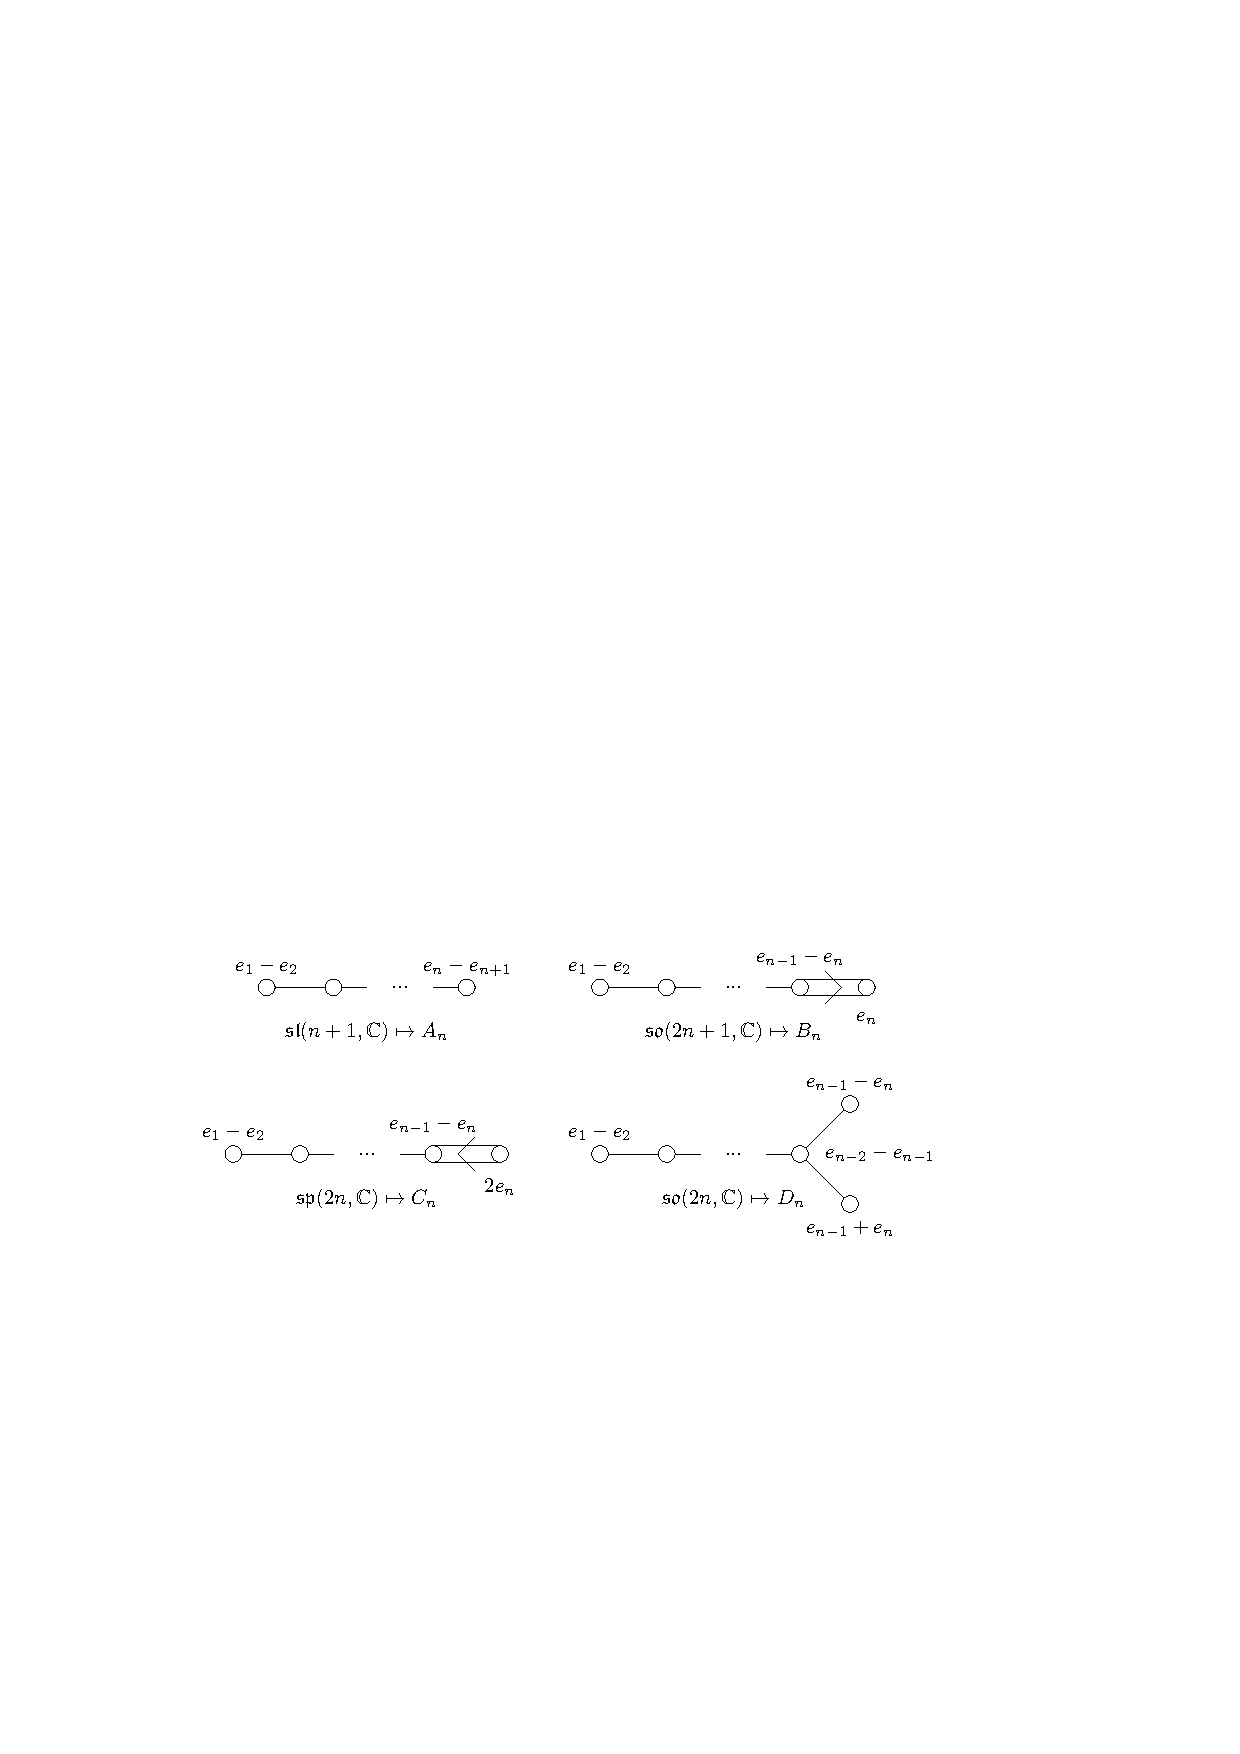
\includegraphics[scale=1]{figures/classical Dynkin diagrams.pdf}
	\end{figure}
	
	\begin{itemize}
		\item $B_2$ and $C_2$, $A_3$ and $D_3$ are isomorphic to each other.
		
		\item $D_2$ 的 Dynkin diagram is not connected $\Longrightarrow$ $D_2$ is reducible $\Longrightarrow \mathfrak{so}(4, \mathbb{C})$ is not simple,
		\begin{equation}
			\mathfrak{so}(4, \mathbb{C}) = \Big( \mathrm{span}(e_1 - e_2) \oplus \mathfrak{g}_{\pm (e_1 - e_2)} \Big) \boldsymbol{\oplus} \Big( \mathrm{span}(e_1 + e_2) \oplus \mathfrak{g}_{\pm (e_1 + e_2)} \Big)
		\end{equation}
		中间粗体的 $\oplus$ 是 Lie algebra direct sum, (两个 $\mathfrak{su}(2)_\mathbb{C}$).
		
		\item $A_n, B_n, C_n, n \geq 1$ 和 $D_n, n \geq 3$ 都对应 simple Lie algebra,
		\begin{equation}
			\begin{array}{cccc}
				\mathfrak{sl}(n + 1, \mathbb{C}) \mapsto A_n & \mathfrak{so}(2 n + 1, \mathbb{C}) \mapsto B_n & \mathfrak{sp}(2 n, \mathbb{C}) \mapsto C_n & \mathfrak{so}(2 n, \mathbb{C}) \mapsto D_n \\
				n \geq 1 & n \geq 1 & n \geq 1 & n \geq 3
			\end{array}
		\end{equation}
	\end{itemize}
\end{itemize}

\subsection{the special linear algebras, \texorpdfstring{$\mathfrak{sl}(n + 1, \mathbb{C}) = \mathfrak{su}(n + 1)_\mathbb{C}$}{sl(n + 1, C) = su(n + 1)\_C}, and \texorpdfstring{$A_n$}{A\_n}}
\begin{itemize}
	\item $\mathfrak{su}(n + 1) = \{A \in \mathcal{M}_{n + 1}(\mathbb{C}) | A^\dag = - A \ \text{and} \ \mathrm{tr} A = 0\}$, 它的 maximal commutative subalgebra 是,
	\begin{equation}
		\mathfrak{t} = \{\mathrm{diag}(i a_1, \cdots, i a_{n + 1}) | a_i \in \mathbb{R} \ \text{and} \ a_1 + \cdots + a_{n + 1} = 0\}
	\end{equation}
	从而得到 Cartan subalgebra, $\mathfrak{h} = \mathfrak{t}_\mathbb{C} = \{\mathrm{diag}(\lambda_1, \cdots, \lambda_{n + 1}) | \lambda_i \in \mathbb{C} \ \text{and} \ \lambda_1 + \cdots + \lambda_{n + 1} = 0\}$.
	
	\noindent\rule[0.5ex]{\linewidth}{0.5pt} % horizontal line
	
	\item 令 $E_{i j}, i \neq j \in \{1, \cdots, n + 1\}$ 是第 $i$ 行第 $j$ 列的分量为 $1$, 其余位置为零的矩阵, $H = \mathrm{diag}(\lambda_1, \cdots) \in \mathfrak{h}$, 那么,
	\begin{equation}
		[H, E_{i j}] = (\lambda_i - \lambda_j) E_{i j}
	\end{equation}
	
	\item 选择一个内积, 使得 $\mathrm{ad}_X, \forall X \in \mathfrak{su}(n + 1)$ 是 skew self-adjoint,
	\begin{equation}
		\braket{A, B} = \mathrm{tr}(A^\dag B), \forall A, B \in \mathfrak{su}(n + 1)_\mathbb{C}
	\end{equation}
	
	\begin{tcolorbox}[title=proof:]
		注意这个内积在任何李代数中都保证 $\mathrm{ad}_X, \forall X \in \mathfrak{k}$ 是 skew self-adjoint, 但是根据 Cartan's criterion, 只有 semisimple 才能保证它 non-degenerate.
		\begin{equation}
			\mathrm{tr}(A^\dag \mathrm{ad}_X B) = \mathrm{tr}(A^\dag X B - A^\dag B X) = \mathrm{tr}(A^\dag X B - X A^\dag B) = \mathrm{tr}(- \mathrm{ad}_X A B)
		\end{equation}
	\end{tcolorbox}
	
	注意, 对于 $H, H' \in \mathfrak{h}$, 有 $\braket{H, H'} = \sum_i \lambda_i^* \lambda'_i$.
	
	\item 可见 $E_{i j}$ 对应的 root 为,
	\begin{equation}
		[H, E_{i j}] = \braket{\underbrace{e_i - e_j}_{= \alpha_{i j}}, H} E_{i j}, i \neq j
	\end{equation}
	
	\noindent\rule[0.5ex]{\linewidth}{0.5pt} % horizontal line
	
	\item $\mathfrak{sl}(n + 1, \mathbb{C})$ 对应的 root system 用 $A_n$ 表示,
	\begin{itemize}
		\item $E = \{v \in \mathbb{R}^{n + 1} | v_1 + \cdots + v_n = 0\}$, 所以 $\dim E = n$.
		
		\item $R = \{\alpha_{i j} = e_i - e_j | i \neq j \in \{1, \cdots, n + 1\}\}$, 共有 $n (n + 1)$ 个根. ($\dim \mathfrak{sl}(n + 1, \mathbb{C}) = (n + 1)^2 - 1$)
		
		\item $\Delta = \{e_1 - e_2, \cdots, e_n - e_{n + 1}\}$ is a base, and $R^+ = \{e_i - e_j | i < j\}$, with,
		\begin{equation}
			e_i - e_j = (e_i - e_{i + 1}) + (e_{i + 1} - e_{i + 2}) + \cdots + (e_{j - 1} - e_j)
		\end{equation}
		
		\item 所有根的长度为 $\sqrt{2}$, 因此 $\braket{\alpha, \beta} = \braket{\alpha, H_\beta}$.
		
		\item $\braket{\alpha, \beta} = 0, \pm 1$ (when $\alpha \neq \pm \beta$).
		
		\item 两个 roots ($\alpha \neq \pm \beta$) 之间的夹角可能是 $\frac{\pi}{2}, \frac{\pi}{3}, \frac{2 \pi}{3}$.
		
		\item 对于 base 中的根, 相邻 (consecutive) 的根夹角为 $\frac{2 \pi}{3}$, 不相邻的互相垂直, 所以其 Dynkin 图如下,
		
		\begin{figure}[H]
			\centering
			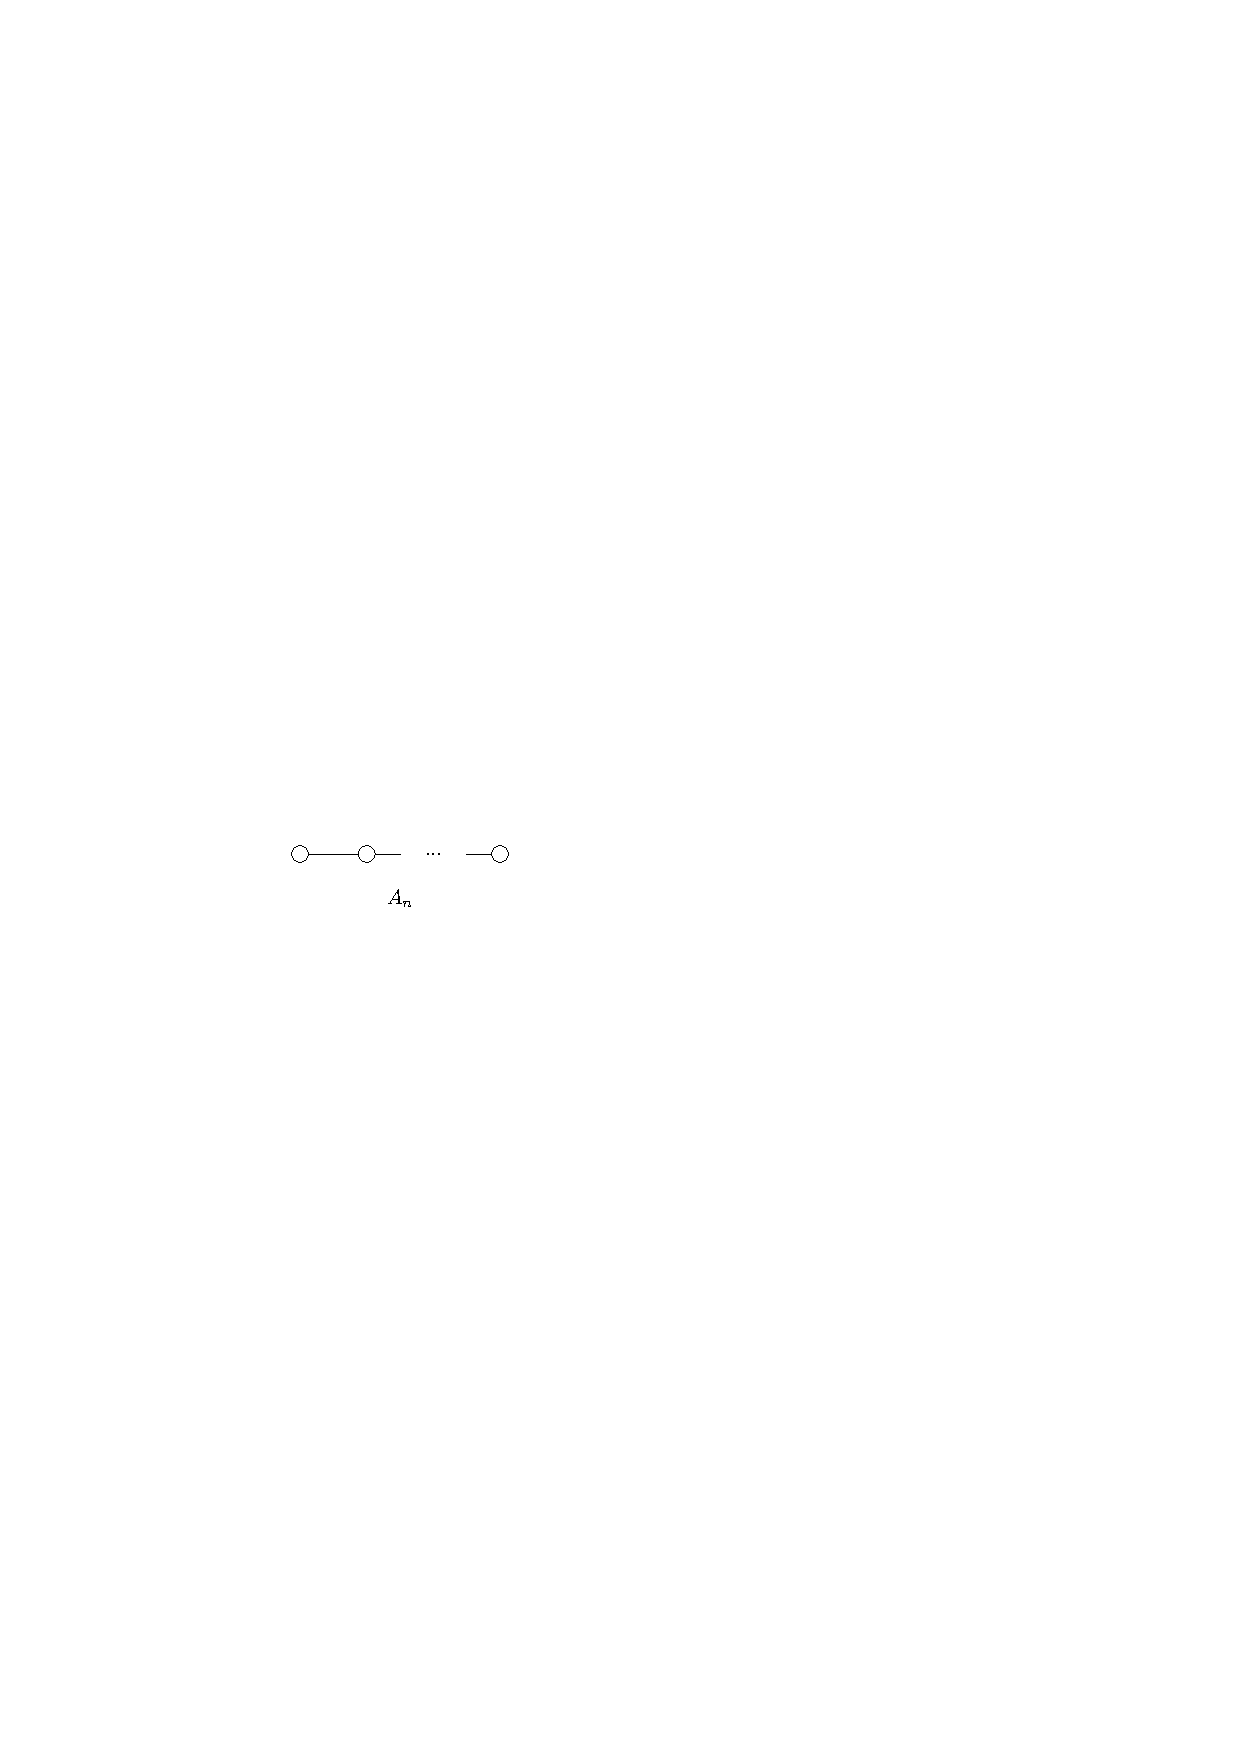
\includegraphics[scale=1]{figures/Dynkin diagram for An.pdf}
		\end{figure}
		
		\item $s_{\alpha_{i j}}$ 作用到向量 $\ket{v}$ 使其 $i, j$ 分量的位置交换, 因此 $A_n$ 的 Weyl 群是 $n + 1$ 个元素的 permutation group.
	\end{itemize}
\end{itemize}

\subsection{the orthogonal algebras, \texorpdfstring{$\mathfrak{so}(2 n, \mathbb{C})$}{so(2 n, C)}, and \texorpdfstring{$D_n$}{D\_n}}
\begin{itemize}
	\item $\mathfrak{so}(2 n, \mathbb{R}) = \mathfrak{o}(2 n, \mathbb{R}) = \{A \in \mathcal{M}_{2 n}(\mathbb{R}) | A^T = - A\}$, 它的 maximal commutative subalgebra 是,
	\begin{equation}
		\mathfrak{t} = \{H_a = \begin{pmatrix}
			0 & a \\
			- a & 0
		\end{pmatrix} | a = \mathrm{diag}(a_1, \cdots, a_n) \ \text{with} \ a_i \in \mathbb{R}\}
	\end{equation}
	
	\begin{tcolorbox}[title=proof:]
		任何 $\mathfrak{so}(2 n, \mathbb{C})$ 中的元素都可以展开成 $\mathfrak{h} = \mathfrak{t}_C$ 和 $D^\alpha_{i j}$ (见下文) 的叠加, 那么, 与 $\mathfrak{h}$ 对易的元素一定不含有 $D^\alpha_{i j}$ 分量, 所以... 是 maximal. (总共有 $2 n^2 - 2 n$ 个根, 且 rank 为 $n$, 所以总维数为 $2 n^2 - n = \frac{2 n (2 n - 1)}{2}$)
		
		另外, 注意如果 $n = 2$, $D^1_{1 1} = D^2_{1 1} = 0$ 而,
		\begin{equation}
			D^3_{1 1} = - D^4_{1 1} = \begin{pmatrix}
				0 & - 2 i \\
				2 i & 0
			\end{pmatrix} \in \mathfrak{h}
		\end{equation}
		也即 $\mathfrak{so}(2, \mathbb{C}) = \mathfrak{h}$, 与不存在 nontrivial center 的对应不符, 不是 semisimple.
	\end{tcolorbox}
	
	\noindent\rule[0.5ex]{\linewidth}{0.5pt} % horizontal line
	
	\item the root vectors are $D^\alpha_{i j} = C^\alpha_{i j} - (C^{\alpha}_{i j})^T$, where $\alpha = 1, 2, 3, 4$ and,
	\begin{align}
		& C^1_{i j} = \begin{pmatrix}
			E_{i j} & i E_{i j} \\
			i E_{i j} & - E_{i j}
		\end{pmatrix} \quad C^2_{i j} = \begin{pmatrix}
			E_{i j} & - i E_{i j} \\
			- i E_{i j} & - E_{i j}
		\end{pmatrix} \notag \\
		& C^3_{i j} = \begin{pmatrix}
			E_{i j} & - i E_{i j} \\
			i E_{i j} & E_{i j}
		\end{pmatrix} \quad C^4_{i j} = \begin{pmatrix}
			E_{i j} & i E_{i j} \\
			- i E_{i j} & E_{i j}
		\end{pmatrix}
	\end{align}
	where $i \neq j \in \{1, \cdots, n\}$ (如果 $i = j$, 那么 $D^{1, 2}_{i i} = 0, D^{3, 4}_{i i} \in \mathfrak{h}$), and we have,
	\begin{align}
		& [H_a, D^1_{i j}] = i (a_i + a_j) D^1_{i j} \quad [H_a, D^2_{i j}] = - i (a_i + a_j) D^2_{i j} \notag \\
		& [H_a, D^3_{i j}] = i (a_i - a_j) D^3_{i j} \quad [H_a, D^4_{i j}] = - i (a_i - a_j) D^4_{i j}
	\end{align}
	
	\begin{tcolorbox}[title=calculation:]
		we have $D^1_{i j} = C^1_{i j} - C^1_{j i}, D^2_{i j} = C^2_{i j} - C^2_{j i}, D^3_{i j} = C^3_{i j} - C^4_{j i}, D^4_{i j} = C^4_{i j} - C^3_{j i}$, and,
		\begin{align}
			& [H_a, C^1_{i j}] = i (a_i + a_j) C^1_{i j} \quad [H_a, C^2_{i j}] = - i (a_i + a_j) C^2_{i j} \notag \\
			& [H_a, C^3_{i j}] = i (a_i - a_j) C^3_{i j} \quad [H_a, C^4_{i j}] = - i (a_i - a_j) C^4_{i j}
		\end{align}
	\end{tcolorbox}
	
	\item 内积定义为 $\braket{A, B} = \frac{1}{2} \mathrm{tr}(A^\dag B)$, 那么,
	\begin{equation}
		\braket{H_a, H_b} = - \sum_{i = 1}^n a_i^* b_i
	\end{equation}
	所以, 可以将 $H_a$ 视作 $i (a_1, \cdots, a_n)$.
	
	\item 可见 root vectors 和 roots 的对应关系为 ($i \neq j \in \{1, \cdots, n\}$),
	\begin{equation}
		D^1_{i j} \mapsto \alpha_{i j} = e_i + e_j \quad D^2_{i j} \mapsto - \alpha_{i j} \quad D^3_{i j} \mapsto \beta_{i j} = e_i - e_j \quad D^4_{i j} \mapsto - \beta_{i j}
	\end{equation}
	
	\noindent\rule[0.5ex]{\linewidth}{0.5pt} % horizontal line
	
	\item $\mathfrak{so}(2 n, \mathbb{C})$ 对应的 root system 用 $D_n$ 表示,
	\begin{itemize}
		\item $E = \mathbb{R}^n$.
		
		\item $R = \{\pm e_i \pm e_j | i \neq j \in \{1, \cdots, n\}\}$, 共有 $\frac{n (n - 1)}{2} \times 4 = 2 n^2 - 2 n$ 个根. ($\dim \mathfrak{so}(2 n, \mathbb{C}) = \frac{2 n (2 n - 1)}{2}$)
		
		\item $\Delta = \{e_1 - e_2, \cdots, e_{n - 1} - e_n\} \cup \{e_{n - 1} \mathcolor{red}{+} e_n\}$ is a base, and $R^+ = \{e_i - e_j | i < j\} \cup \{e_i + e_j\}$, with,
		\begin{equation}
			e_i + e_j = \underbrace{(e_i - e_{i + 1}) + \cdots + (e_{n - 1} + e_n)}_{= e_i + e_n} + \underbrace{(e_j - e_{j + 1}) + \cdots + (e_{n - 1} - e_n)}_{= e_j - e_n}
		\end{equation}
		
		\item 所有根的长度为 $\sqrt{2}$, 因此也有 $\braket{\alpha, \beta} = \braket{\alpha, H_\beta}$.
		
		\item $\braket{\alpha, \beta} = 0, \pm 1$ (when $\alpha \neq \pm \beta$), 所以两个根之间的夹角可能是 $\frac{\pi}{2}$ 或 $\frac{\pi}{3}, \frac{2 \pi}{3}$.
		
		\item $D_n$ 的 Dynkin 图如下,
		
		\begin{figure}[H]
			\centering
			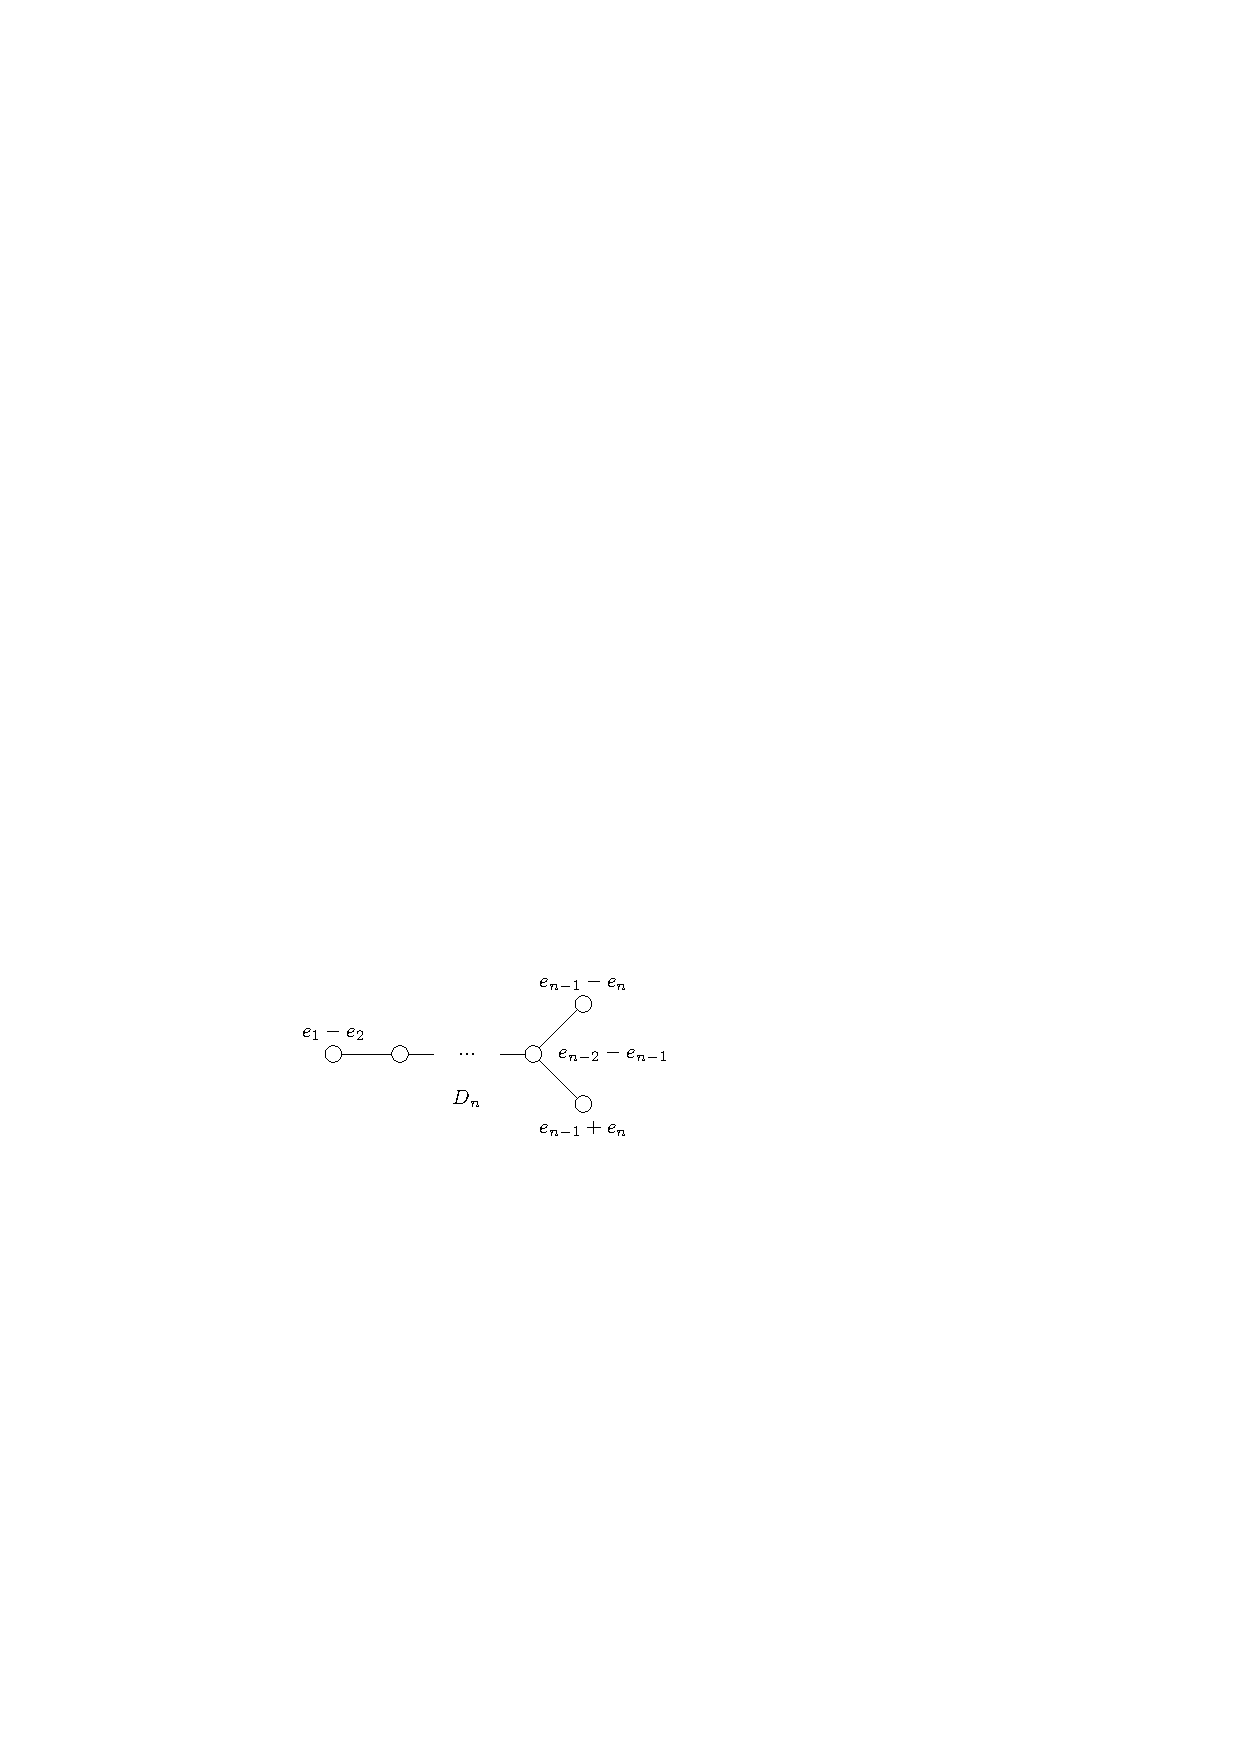
\includegraphics[scale=1]{figures/Dynkin diagram for Dn.pdf}
		\end{figure}
		
		\item $s_\alpha = s_{- \alpha}, \alpha \in R$ 分别为,
		\begin{equation}
			\begin{dcases}
				s_{\alpha_{i j}} : (\cdots, v_i, \cdots, v_j, \cdots) \mapsto (\cdots, - v_j, \cdots, - v_i, \cdots) \\
				s_{\beta_{i j}} : (\cdots, v_i, \cdots, v_j, \cdots) \mapsto (\cdots, v_j, \cdots, v_i, \cdots)
			\end{dcases}
		\end{equation}
	\end{itemize}
\end{itemize}

\subsection{the orthogonal algebras, \texorpdfstring{$\mathfrak{so}(2 n + 1, \mathbb{C})$}{so(2 n + 1, C)}, and \texorpdfstring{$B_n$}{B\_n}}
\begin{itemize}
	\item its maximal commutative subalgebra is,
	\begin{equation}
		\mathfrak{t} = \{\left( \begin{array}{cc|c}
			0 & a & \\
			- a & 0 & \\
			\hline
			& & 0
		\end{array} \right) | a = \mathrm{diag}(a_1, \cdots, a_n) \ \text{with} \ a_i \in \mathbb{R}\}
	\end{equation}
	both $\mathfrak{so}(2 n + 1, \mathbb{C})$ and $\mathfrak{so}(2 n, \mathbb{C})$ have rank $n$.
	
	\noindent\rule[0.5ex]{\linewidth}{0.5pt} % horizontal line
	
	\item every root in $\mathfrak{so}(2 n, \mathbb{C})$ is a root in $\mathfrak{so}(2 n + 1, \mathbb{C})$, but there are $2 n$ additional roots in $\mathfrak{so}(2 n + 1, \mathbb{C})$.
	
	\item the additional root vectors are,
	\begin{equation}
		B^1_k = \left( \begin{array}{ccc|ccc|c}
			& & & & & & \vdots \\
			& & & & & & 1 \\
			& & & & & & \vdots \\
			\hline
			& & & & & & \vdots \\
			& & & & & & i \\
			& & & & & & \vdots \\
			\hline
			\cdots & - 1 & \cdots & \cdots & - i & \cdots & 0
		\end{array} \right) \quad B^2_k = \left( \begin{array}{ccc|ccc|c}
			& & & & & & \vdots \\
			& & & & & & 1 \\
			& & & & & & \vdots \\
			\hline
			& & & & & & \vdots \\
			& & & & & & - i \\
			& & & & & & \vdots \\
			\hline
			\cdots & - 1 & \cdots & \cdots & i & \cdots & 0
		\end{array} \right)
	\end{equation}
	其中 $B^{1, 2}_k$ 的非零元素位于 $(k, 2 n + 1), (n + k, 2 n + 1)$ 和通过转置相对应的位置, 有对易关系,
	\begin{equation}
		[H_a, B^1_k] = i a_k B^1_k \quad [H_a, B^2_k] = - i a_k B^2_k
	\end{equation}
	
	\item 选取与上一 subsection 一样的内积, 那么 root vectors 和 roots 的对应关系为,
	\begin{equation}
		B^1_k \mapsto e_k \quad B^2_k \mapsto - e_k
	\end{equation}
	
	\noindent\rule[0.5ex]{\linewidth}{0.5pt} % horizontal line
	
	\item $\mathfrak{so}(2 n + 1, \mathbb{C})$ 对应的 root system 用 $B_n$ 表示,
	\begin{itemize}
		\item $E = \mathbb{R}^n$.
		
		\item $R = \{\pm e_i \pm e_j \ \text{and} \ \pm e_k | i \neq j, k \in \{1, \cdots, n\}\}$, 共有 $2 n^2$ 个根. ($\dim \mathfrak{so}(2 n + 1, \mathbb{C}) = \frac{(2 n + 1) 2 n}{2}$)
		
		\item $\Delta = \{e_1 - e_2, \cdots, e_{n - 1} - e_n\} \cup \{e_n\}$ is a base, and $R^+ = \{e_i - e_j | i < j\} \cup \{e_i + e_j\} \cup \{e_k\}$.
		
		\item $\braket{\alpha, \beta} = 0, \pm 1$ (when $\alpha \neq \pm \beta$), 所以两个根之间的夹角可能为 $\frac{\pi}{2}, \frac{\pi}{3}, \frac{2 \pi}{3}, \frac{\pi}{4}, \frac{3 \pi}{4}$.
		
		\item $B_n$ 的 Dynkin 图如下,
		
		\begin{figure}[H]
			\centering
			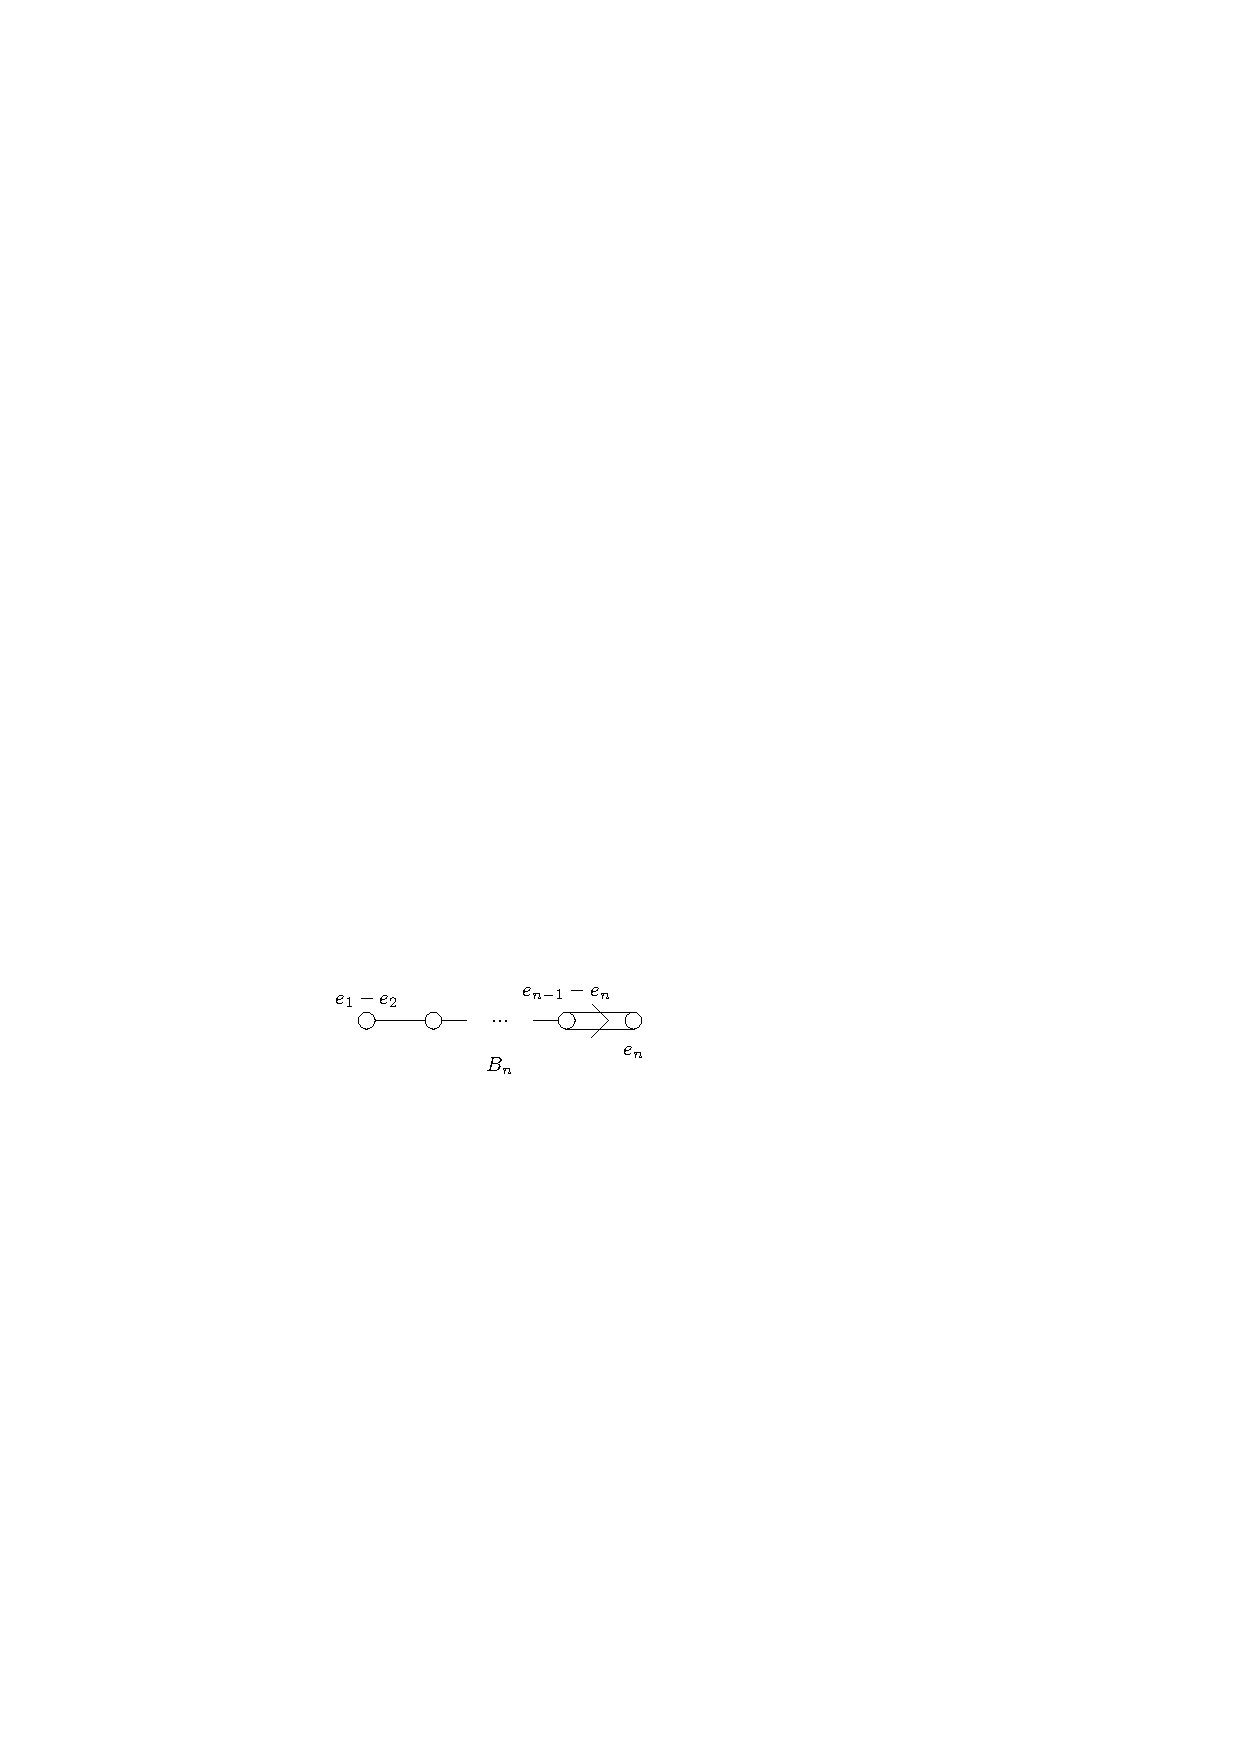
\includegraphics[scale=1]{figures/Dynkin diagram for Bn.pdf}
		\end{figure}
	\end{itemize}
\end{itemize}

\subsection{the symplectic algebras, \texorpdfstring{$\mathfrak{sp}(2 n, \mathbb{C})$}{sp(2 n, C)}, and \texorpdfstring{$C_n$}{C\_n}}
\begin{itemize}
	\item $\mathfrak{sp}(2 n, \mathbb{C}) = \{A \in \mathcal{M}_{2 n}(\mathbb{C}) | \Omega A^T \Omega = A\}$, where,
	\begin{equation}
		\Omega = \begin{pmatrix}
			0 & I \\
			- I & 0
		\end{pmatrix}
	\end{equation}
	$\mathfrak{sp}(2 n, \mathbb{C})$ 中的矩阵可以写成如下形式,
	\begin{equation}
		A = \begin{pmatrix}
			a & b \\
			c & - a^T
		\end{pmatrix}
	\end{equation}
	where $a, b, c \in \mathcal{M}_n(\mathbb{C})$, and $b, c$ are symmetric.
	
	\item 可以认为 $\mathfrak{k} = \mathfrak{sp}(2 n, \mathbb{C}) \cap \mathfrak{u}(2 n)$ 是其 compact real form,
	\begin{equation}
		\mathfrak{sp}(2 n, \mathbb{C}) \cap \mathfrak{u}(2 n) = \{\begin{pmatrix}
			a & b \\
			- b^\dag & - a^T
		\end{pmatrix} | a^\dag = - a, b^T = b\}
	\end{equation}
	
	\item the maximal commutative subalgebra of $\mathfrak{k}$ is,
	\begin{equation}
		\mathfrak{t} = \{H_a = \begin{pmatrix}
			a & 0 \\
			0 & - a
		\end{pmatrix} | a = \mathrm{diag}(a_1, \cdots, a_n), \mathcolor{red}{i} a_i \in \mathbb{R}\}
	\end{equation}
	
	\noindent\rule[0.5ex]{\linewidth}{0.5pt} % horizontal line
	
	\item the root vectors are ($i \neq j$),
	\begin{align}
		& A_{i j} = \begin{pmatrix}
			0 & E_{i j} + E_{j i} \\
			0 & 0
		\end{pmatrix} \quad B_{i j} = \begin{pmatrix}
			0 & 0 \\
			E_{i j} + E_{j i} & 0
		\end{pmatrix} \quad C_{i j} = \begin{pmatrix}
			E_{i j} & 0 \\
			0 & - E_{j i}
		\end{pmatrix} \notag \\
		& F_k = \begin{pmatrix}
			0 & E_{k k} \\
			0 & 0
		\end{pmatrix} \quad G_k = \begin{pmatrix}
			0 & 0 \\
			E_{k k} & 0
		\end{pmatrix}
	\end{align}
	对易关系为,
	\begin{align}
		& [H_a, A_{i j}] = (a_i + a_j) A_{i j} \quad [H_a, B_{i j}] = - (a_i + a_j) B_{i j} \quad [H_a, C_{i j}] = (a_i - a_j) C_{i j} \notag \\
		& [H_a, F_k] = 2 a_k F_k \quad [H_a, G_k] = - 2 a_k G_k
	\end{align}
	
	\item 选取内积为 $\braket{A, B} = \frac{1}{2} \mathrm{tr}(A^\dag B)$, 所以 $H_a$ 可以视为 $(a_1, \cdots, a_n)$, 那么 root vectors 和 roots 的对应关系为,
	\begin{equation}
		A_{i j} \mapsto e_i + e_j \quad B_{i j} \mapsto - e_i - e_j \quad C_{i j} \mapsto e_i - e_j \quad F_k \mapsto 2 e_k \quad G_k \mapsto - 2 e_k
	\end{equation}
	
	\noindent\rule[0.5ex]{\linewidth}{0.5pt} % horizontal line
	
	\item $\mathfrak{sp}(2 n, \mathbb{C})$ 对应的 root system 用 $C_n$ 表示,
	\begin{itemize}
		\item $E = \mathbb{R}^n$.
		
		\item $R = \{\pm e_i \pm e_j \ \text{and} \ \pm 2 e_k | i \neq j, k \in \{1, \cdots, n\}\}$, 与 $B_n$ 相似 (区别是 $\pm e_k$ 前的系数 $2$), 共有 $2 n^2$ 个根. ($\dim \mathfrak{sp}(2 n, \mathbb{C}) = n (2 n + 1)$)
		
		\item $\Delta = \{e_1 - e_2, \cdots, e_{n - 1} - e_n\} \cup \{2 e_n\}$ and $R = \{e_i - e_j | i < j\} \cup \{e_i + e_j\} \cup \{2 e_k\}$.
		
		\item $\braket{\alpha, \beta} = 0, \pm 1, \pm 2$ (when $\alpha \neq \pm \beta$), 所以两个根之间夹角可能为 $\frac{\pi}{2}, \frac{\pi}{3}, \frac{2 \pi}{3}, \frac{\pi}{4}, \frac{3 \pi}{4}$.
		
		\item $C_n$ 的 Dynkin 图如下,
		
		\begin{figure}[H]
			\centering
			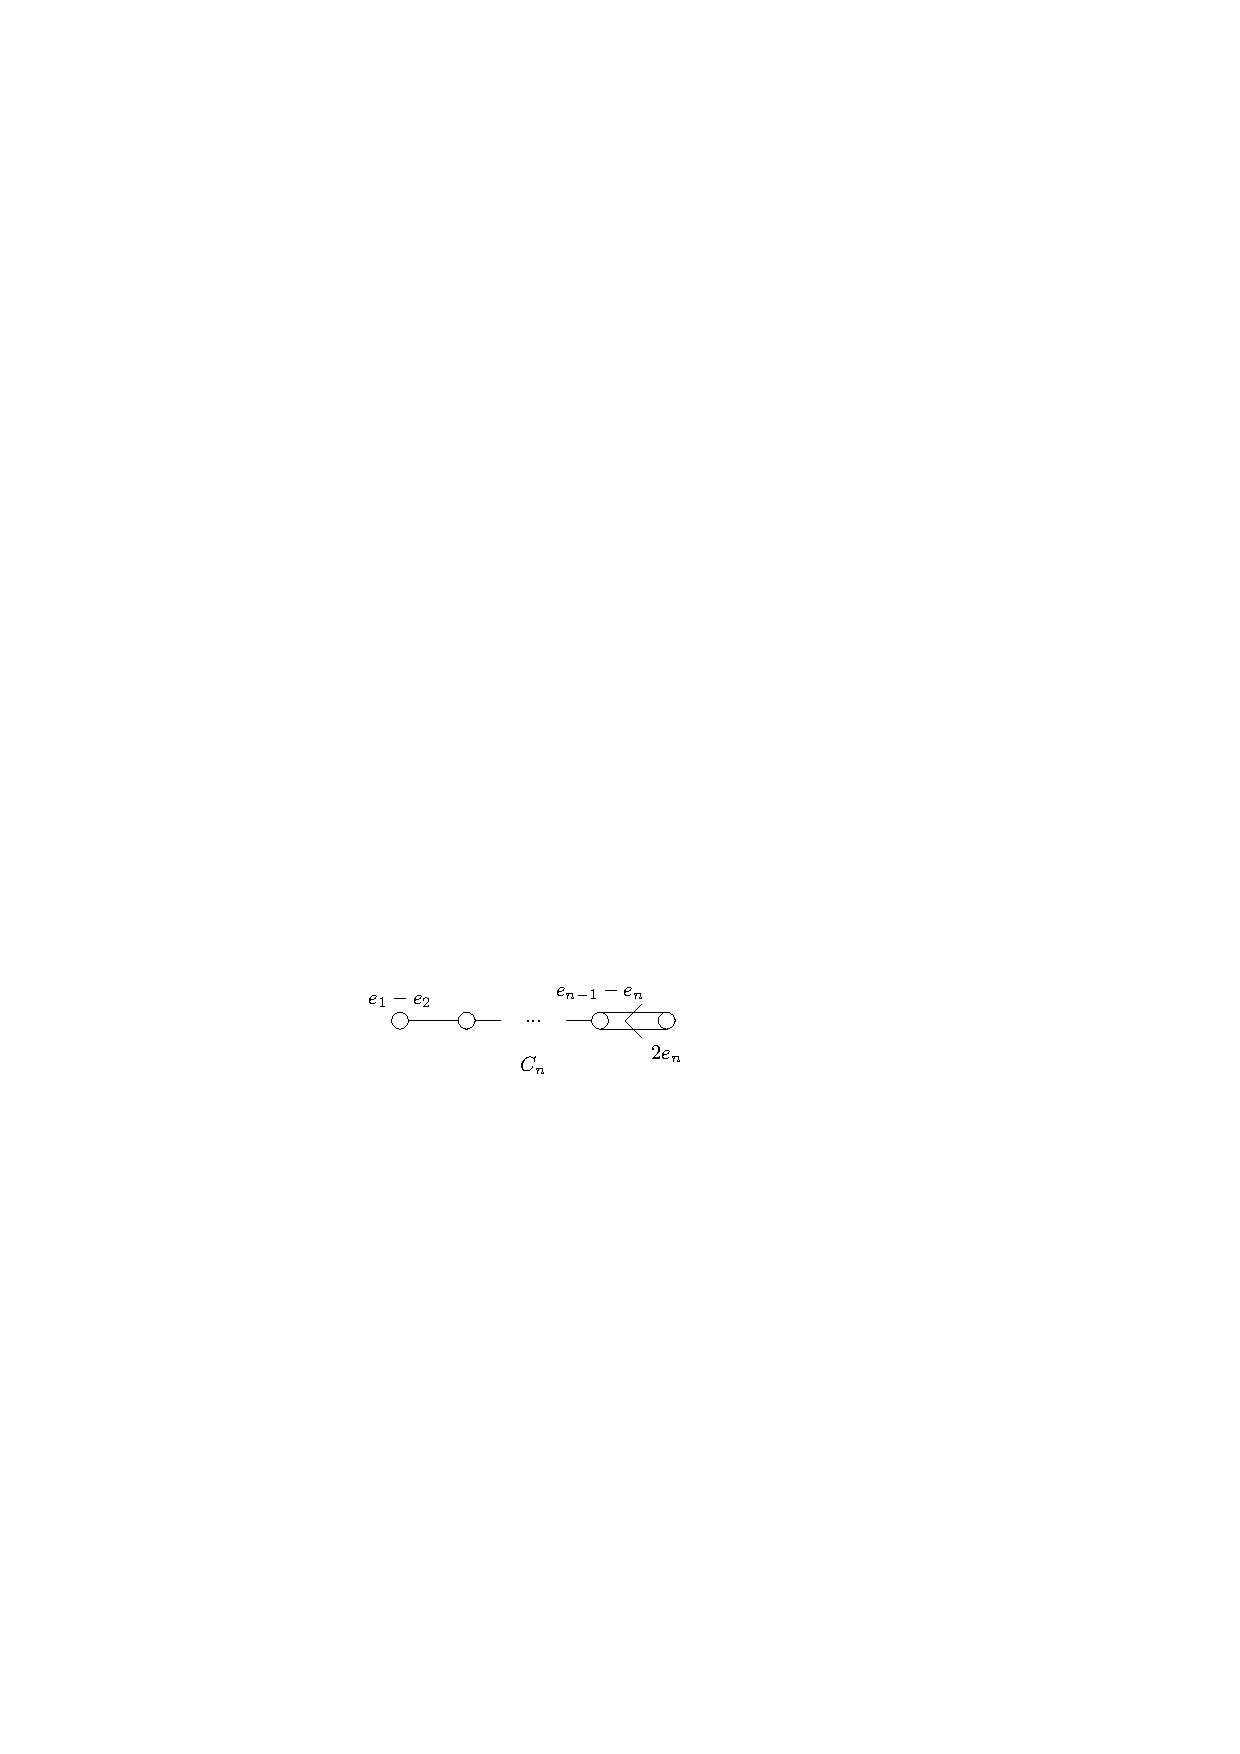
\includegraphics[scale=1]{figures/Dynkin diagram for Cn.pdf}
		\end{figure}
	\end{itemize}
\end{itemize}
